%% demo.tex
%% Copyright 2017 Pietro Saccardi (saccardi at or.uni-bonn.de)
%
% This work may be distributed and/or modified under the
% conditions of the LaTeX Project Public License, either version 1.3
% of this license or (at your option) any later version.
% The latest version of this license is in
%   http://www.latex-project.org/lppl.txt
% and version 1.3 or later is part of all distributions of LaTeX
% version 2005/12/01 or later.
%
% This work has the LPPL maintenance status `maintained'.
%
% The Current Maintainer of this work is Pietro Saccardi.
%
% This work consists of the files bigsposter.cls, demo.tex, instruction.pdf.

\documentclass[a2paper]{bigsposter}
\usepackage{lipsum}
\usepackage[utf8]{inputenc}
\usepackage{algorithm}
\usepackage{algorithmic}
\usepackage{comment}
\usepackage{xcolor}
\usepackage{setspace}
\definecolor{mustardyellow}{RGB}{255, 219, 88}
\definecolor{customviolet}{RGB}{143, 0, 255}
\author{Heinz, Paula}
\advisor{Prof.\ Dr.\ Stephan Held}
\title{Congestion-\& Timing-Aware Pin Assignment with Multiply-Instantiated Blocks}
\posteryear{2025}
\email{heinz@dm.uni-bonn.de}
\institute{Research Institute for Discrete Mathematics}

% This is just for making the picture placeholder
\newcommand{\emptybox}[2]{\framebox[#1]{\rule{0pt}{#2}}}


% This is just for putting the bibliography in a single file
\bibliographystyle{alpha}
\begin{filecontents}{samplebib.bib}
@article{samplearticle,
  author={E\'variste Galois},
  title={M\'emoire sur les conditions de r\'esolubilit\'e des \'equations par radicaux},
  year={1831}
}
@inproceedings{AlbrechtKMZ02,
	author = {Albrecht, C. and Kahng, A.B. and Mandoiu, I. and Zelikovsky, A.},
	booktitle = {ASP-DAC},
	pages = {580--587},
	title = {Floorplan evaluation with timing-driven global wireplanning, pin assignment and buffer/wire sizing},
	year = 2002
}

@inproceedings{BatterywalaTrackAssign,
	author = {Batterywala, S. and Shenoy, N. and Nicholls, W. and Zhou, H.},
	booktitle = {IEEE/ACM International Conference on Computer Aided Design, 2002. ICCAD 2002.},
	doi = {10.1109/ICCAD.2002.1167514},
	issn = {1092-3152},
	keywords = {VLSI; circuit layout CAD; crosstalk; integrated circuit interconnections; integrated circuit layout; network routing; back-end design process; connectivity; cost metrics; cross-talk; detailed routing; global routing; intermediate track assignment heuristic; lookahead heuristic; process constraints; routing algorithms; segment splitting heuristic; signal delay; signal integrity; three stage routing process; track assignment; weighted bipartite matching heuristic; wiring completions; Costs; Crosstalk; Delay; Pins; Process design; Routing; Signal processing; Very large scale integration; Wire; Wiring},
	month = {Nov},
	number = {},
	pages = {59--66},
	title = {Track assignment: a desirable intermediate step between global routing and detailed routing},
	volume = {},
	year = 2002
}

@phdthesis{bihler-dissertation,
	author = {Tilmann Bihler},
	title = {Dynamic Local Usage in BonnRouteGlobal},
	school = {Rheinische Friedrich-Wilhelms-Universität Bonn},
	year = 2023,
	url = {https://hdl.handle.net/20.500.11811/11185},
}

@articel{brady1984approach,
	author = {Brady, H Nelson},
	journal = {IEEE transactions on computer-aided design of integrated circuits and systems},
	number = {3},
	pages = {250--255},
	publisher = {IEEE},
	title = {An approach to topological pin assignment},
	volume = {3},
	year = 1984
}

@article{BRGTiming2,
	author = {Held, Stephan and M{\"u}ller, Dirk and Rotter, Daniel and Scheifele, Rudolf and Traub, Vera and Vygen, Jens},
	doi = {10.1109/TCAD.2017.2697964},
	journal = {IEEE Transactions on Computer-Aided Design of Integrated Circuits and Systems},
	number = {2},
	pages = {406--419},
	title = {Global Routing With Timing Constraints},
	volume = {37},
	year = {2018}
}

@inproceedings{Chen+IntegratedFloorplanningAndInterconnectPlanning:1999,
	acmid = {340039},
	address = {Piscataway, NJ, USA},
	author = {Chen, H.-M. and Zhou, H. and Young, F. Y. and Wong, D. F. and Yang, H. H. and Sherwani, N.},
	booktitle = {Proceedings of the 1999 IEEE/ACM International Conference on Computer-aided Design},
	isbn = {0-7803-5832-5},
	location = {San Jose, California, USA},
	numpages = {4},
	pages = {354--357},
	publisher = {IEEE Press},
	series = {ICCAD '99},
	title = {Integrated Floorplanning and Interconnect Planning},
	url = {http://dl.acm.org/citation.cfm?id=339492.340039},
	year = 1999
}

@inproceedings{ChenTY-SALT-ICCAD2017,
	author = {Chen, Gengjie and Tu, Peishan and Young, Evangeline FY},
	booktitle = {Proceedings of the 36th International Conference on Computer-Aided Design},
	organization = {IEEE Press},
	pages = {569--576},
	title = {SALT: provably good routing topology by a novel steiner shallow-light tree algorithm},
	year = 2017
}

@article{cong1991pin,
	author = {Cong, Jason},
	journal = {IEEE transactions on computer-aided design of integrated circuits and systems},
	number = {11},
	pages = {1401--1412},
	publisher = {IEEE},
	title = {Pin assignment with global routing for general cell designs},
	volume = {10},
	year = 1991
}

@inproceedings{CongPinAssignmentICCAD89,
	author = {Cong, J.},
	booktitle = {1989 IEEE International Conference on Computer-Aided Design. Digest of Technical Papers},
	doi = {10.1109/ICCAD.1989.76958},
	issn = {},
	keywords = {VLSI; circuit layout CAD; BeauticianGR; VLSI circuits; algorithm; finite interval decomposition theorem; global routing; global routing step; physical design; pin assignment step; Algorithm design and analysis; Circuits; Computer science; Logic functions; Packaging; Partitioning algorithms; Process design; Routing; Topology; Very large scale integration},
	month = {Nov},
	number = {},
	pages = {302--305},
	title = {Pin assignment with global routing},
	volume = {},
	year = 1989
}

@report{duran:2024,
	author = {Durán Fernández, Victoria},
	title = {Infeasibility Minimization in Track Assignment},
	year = {2024},
	institution = {Research Institute for Discrete Mathematics},
	number = {241307},
	note = {Bachelor thesis},
}

@inproceedings{HeldR-ExactDelayBoundedSteiner18,
	author = {left out for blind review}
}

@inproceedings{Hong+FARM-DAC92,
	acmid = {149625},
	address = {Los Alamitos, CA, USA},
	author = {Hong, X.-L. and Huang, J. and Cheng, C.-K. and Kuh, E. S.},
	booktitle = {Proceedings of the 29th ACM/IEEE Design Automation Conference},
	isbn = {0-89791-516-X},
	location = {Anaheim, California, USA},
	numpages = {6},
	pages = {530--535},
	publisher = {IEEE Computer Society Press},
	series = {DAC '92},
	title = {FARM: An Efficient Feed-through Pin Assignment Algorithm},
	url = {http://dl.acm.org/citation.cfm?id=113938.149625},
	year = 1992
}

@article{JiaMCFDetailedRouter,
	author = {Jia, X. and Cai, Y. and Zhou, Q. and Yu, B.},
	doi = {10.1109/TCAD.2017.2693270},
	issn = {0278-0070},
	journal = {IEEE Transactions on Computer-Aided Design of Integrated Circuits and Systems},
	keywords = {VLSI; circuit optimisation; computational complexity; integer programming; integrated circuit design; linear programming; network routing; DRC violations; NP-hard model; complex design rule constraints; concurrent detailed routing algorithm; efficient acceleration techniques; efficient model solving algorithms; incremental detailed router; integer linear programming; low routing quality; model simplification heuristics; multicommodity flow model; multicommodity flow-based detailed router; nonoptimal net-ordering nature; physical design; routing completion; sequential methods; transistor feature size; very large scale integrated physical design; Algorithm design and analysis; Industries; Layout; Routing; Runtime; Timing; Very large scale integration; Design rules; detailed routing; integer linear programing; multicommodity flow (MCF)},
	month = {Jan},
	number = {1},
	pages = {217--230},
	title = {A Multicommodity Flow-Based Detailed Router With Efficient Acceleration Techniques},
	volume = {37},
	year = 2018
}

@patent{kazda+pangea:21,
	author = {Kazda, M. and Folberth, H. and Villarrubia, P.G. and Held, S. and Saccardi, P.},
	note = {US Patent 1\,108\,045\,6B2},
	title = {Automated design closure with abutted hierarchy},
	year = {2021}
}

@article{KoideWY-PinAssignmentWithGLobalRouting96,
	author = {Koide, T. and Wakabayashi, S. and Yoshida, N.},
	journal = {IEEE transactions on computer-aided design of integrated circuits and systems},
	number = {12},
	pages = {1575--1583},
	publisher = {IEEE},
	title = {Pin assignment with global routing for VLSI building block layout},
	volume = {15},
	year = 1996
}

@inproceedings{koren1972pin,
	author = {Koren, Norman L},
	booktitle = {Proceedings of the 9th Design Automation Workshop},
	organization = {ACM},
	pages = {72--79},
	title = {Pin assignment in automated printed circuit board design},
	year = 1972
}

@article{liu1999multilayer,
	author = {Liu, L-CE and Sechen, Carl},
	journal = {IEEE Transactions on Computer-Aided Design of Integrated Circuits and Systems},
	number = {10},
	pages = {1452--1461},
	publisher = {IEEE},
	title = {Multilayer pin assignment for macro cell circuits},
	volume = {18},
	year = 1999
}

@inproceedings{meister2008novel,
	author = {Meister, Tilo and Lienig, Jens and Thomke, Gisbert},
	booktitle = {Proceedings of the conference on Design, automation and test in Europe},
	organization = {ACM},
	pages = {837--842},
	title = {Novel pin assignment algorithms for components with very high pin counts},
	year = 2008
}

@article{MinMaxResSh,
	author = {M{\"u}ller, Dirk and Radke, Klaus and Vygen, Jens},
	day = {01},
	doi = {10.1007/s12532-011-0023-y},
	issn = {1867-2957},
	journal = {Mathematical Programming Computation},
	month = {Mar},
	number = {1},
	pages = {1--35},
	title = {Faster min--max resource sharing in theory and practice},
	url = {https://doi.org/10.1007/s12532-011-0023-y},
	volume = {3},
	year = 2011
}

@article{nair+berman+hauge+yoffa:1989,
	author = {Nair, R. and Berman, C. L. and Hauge, P. S. and Yoffa, E. J.},
	journal = {IEEETCAD: IEEE Transactions on Computer-Aided Design of Integrated Circuits and Systems},
	pages = {860--874},
	title = {Generation of Performance Constraints for Layout},
	volume = {8},
	year = 1989
}

@article{papa2008rumble,
	title={RUMBLE: An incremental timing-driven physical-synthesis optimization algorithm},
	author={Papa, David A and Luo, Tao and Moffitt, Michael D and Sze, CN and Li, Zhuo and Nam, Gi-Joon and Alpert, Charles J and Markov, Igor L},
	journal={IEEE Transactions on Computer-Aided Design of Integrated Circuits and Systems},
	year={2008}
}

@inproceedings{pedram1990floorplanning,
	author = {Pedram, Massoud and Marek-Sadowska, Malgorzata and Kuh, Ernest S},
	booktitle = {Computer-Aided Design, 1990. ICCAD-90. Digest of Technical Papers., 1990 IEEE International Conference on},
	organization = {IEEE},
	pages = {98--101},
	title = {Floorplanning with pin assignment},
	year = 1990
}

@inproceedings{prasad2009simultaneous,
	author = {Prasad, Shashank and Kumar, Anuj},
	booktitle = {VLSI Design, 2009 22nd International Conference on},
	organization = {IEEE},
	pages = {399--403},
	title = {Simultaneous Routing and Feedthrough Algorithm to Decongest Top Channel},
	year = 2009
}

@thesis{RulandTA2013,
	author = {left out for blind review}
}

@article{RWSCEMMagmaARM08,
	author = {Riches, S. and Watson, P. and Schultz, J. and Churchill, P and Eerappa, S. and Madabushi, V.},
	journal = {ARM Information Quaterly Magazine},
	number = {3},
	title = {Accelerating Hierarchical Implementation of the ARM Cortex-A9 with Magma{\rq}s Hydra},
	volume = {7},
	year = 2008
}

@incollection{Scheffer-IndustrialFloorplanningAndPrototyping08,
	author = {Scheffer, Louis K.},
	bibsource = {dblp computer science bibliography, https://dblp.org},
	biburl = {https://dblp.org/rec/bib/reference/crc/Scheffer08},
	booktitle = {Handbook of Algorithms for Physical Design Automation.},
	doi = {10.1201/9781420013481.ch13},
	timestamp = {Wed, 12 Jul 2017 09:11:51 +0200},
	title = {Industrial Floorplanning and Prototyping},
	url = {https://doi.org/10.1201/9781420013481.ch13},
	year = 2008
}

@inproceedings{ShallowLight,
	address = {Berlin, Heidelberg},
	author = {Held, Stephan and Rotter, Daniel},
	booktitle = {Integer Programming and Combinatorial Optimization},
	editor = {Goemans, Michel and Correa, Jos{\'e}},
	isbn = {978-3-642-36694-},
	pages = {229--241},
	publisher = {Springer Berlin Heidelberg},
	title = {Shallow-Light Steiner Arborescences with Vertex Delays},
	year = 2013
}

@inproceedings{ShiDavoodiTrackPlanning,
	author = {Shi, D. and Davoodi, A.},
	booktitle = {2017 54th ACM/EDAC/IEEE Design Automation Conference (DAC)},
	doi = {10.1145/3061639.3062335},
	issn = {},
	keywords = {integrated circuit design; network routing; global routing stage; local congestion track planning; track assignment algorithm; track congestion; Optimization; Planning; Routing; Tools; Tracking; Very large scale integration},
	month = {June},
	number = {},
	pages = {1--6},
	title = {TraPL: Track planning of local congestion for global routing},
	volume = {},
	year = 2017
}

@inproceedings{wang1991simultaneous,
	author = {Wang, LY and Lai, YT and Liu, BD},
	booktitle = {Circuits and Systems, 1991., IEEE International Sympoisum on},
	organization = {IEEE},
	pages = {2128--2131},
	title = {Simultaneous pin assignment and global wiring for custom VLSI design},
	year = 1991
}

@inproceedings{WeiLCHAS13,
	author = {Wei, Y. and Li, Z. and Sze, C.C.N. and Hu, S. and Alpert, C.J. and S.S., Sapatnekar},
	booktitle = {DATE},
	pages = {1873--1878},
	title = {CATALYST: planning layer directives for effective design closure},
	year = 2013
}

@inproceedings{WongNegotiationTrackAssign,
	author = {Wong, M. P. and Liu, W. H. and Wang, T. C.},
	booktitle = {2016 21st Asia and South Pacific Design Automation Conference (ASP-DAC)},
	doi = {10.1109/ASPDAC.2016.7428041},
	issn = {},
	keywords = {VLSI; integrated circuit design; network routing; VLSI design flow; global routing; iroutes; local nets; negotiation-based track assignment; track-assignment-based routability estimator; Wiring},
	month = {Jan},
	number = {},
	pages = {378--383},
	title = {Negotiation-based track assignment considering local nets},
	volume = {},
	year = 2016
}

@article{xiang2003min,
	author = {Xiang, Hua and Tang, Xiaoping and Wong, Martin DF},
	journal = {IEEE Transactions on Computer-Aided Design of Integrated Circuits and Systems},
	number = {7},
	pages = {870--878},
	publisher = {IEEE},
	title = {Min-cost flow-based algorithm for simultaneous pin assignment and routing},
	volume = {22},
	year = 2003
}

@article{xiang2005algorithm,
	author = {Xiang, Hua and Tang, Xiaoping and Wong, Martin DF},
	journal = {ACM Transactions on Design Automation of Electronic Systems (TODAES)},
	number = {3},
	pages = {561--572},
	publisher = {ACM},
	title = {An algorithm for integrated pin assignment and buffer planning},
	volume = {10},
	year = 2005
}


\end{filecontents}

\begin{document}

  \maketitle
  \begin{blockrow}[3]
    \blocktitle{Port Assignment without Reuse Blocks}
    	\begin{minipage}{0.45\blockwidth}
    	 Large integrated circuits are often partitioned into multiple blocks
    	to reduce tool running times and  parallelize the design process. Port
    	assignment defines positions and shapes for the interface pins of the
    	blocks. It has a big impact on signal speeds and routability.
    
    
    \end{minipage}\hspace{0.09\blockwidth}%
    \begin{minipage}{0.45\blockwidth}
    	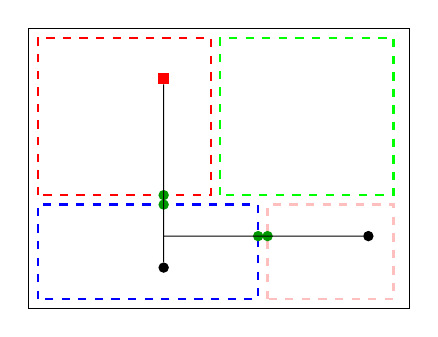
\begin{tikzpicture}[scale=0.4]
    		\draw[thick,dashed,blue] (0,1) rectangle ++ (7,3);
    		\draw[thick,dashed,red] (0,4.3) rectangle ++ (5.5,5);
    		\draw[thick,dashed,green] (5.8,4.3) rectangle ++ (5.5,5);
    		\draw[thick,dashed,pink] (7.3,1) rectangle ++ (4,3);
    		\draw[black] (-0.3,0.7) rectangle ++ (12.1,8.9);
    		
    		\node[fill=red, scale=0.6] (root) at (4,8){};
    		\node[shape=circle,fill=black,scale=0.4] (sink) at (10.5,3){};
    		\node[shape=circle,fill=black,scale=0.4] (sink2) at (4,2){};
    		
    		\node[shape=circle,fill=green!60!black,scale=0.4] (port1) at (7,3){};
    		\node[shape=circle,fill=green!60!black,scale=0.4] (port3) at (4,4){};
    		\node[shape=circle,fill=green!60!black,scale=0.4] (port4) at (4,4.3){};
    		\node[shape=circle,fill=green!60!black,scale=0.4] (port2) at (7.3,3){};
    		
    		\draw[-] (4,3) -- (port2) -- (port1) -- (sink);
    		\draw[-] (root)  -- (port3) -- (port4) -- (sink2);
    	\end{tikzpicture}
    \end{minipage}\\

 \label{sec:modfied_global;_routing}
 The goal is to achieve a pin assignment with the following properties:
 \begin{enumerate}
 	\item \textbf{low inter-block dependency} (i.e. few ports)
 	\item \textbf{enable fast signals} (ports lying on shortest source-to-sink path)
 	\item \textbf{short total net length/small power consumption}
 	\item \textbf{prevent routing congestion} (ports spread out)
 \end{enumerate}
 BonnPangea is tailored but not limited to a setting, where the
 circuit is sliced into almost abutting blocks that ``own'' the
 complete metal stack above their area, which is employed for example
 on IBM microprocessors \cite{kazda+pangea:21}.
Our general approach for pin assignment is to run global routing with
global static timing constraints \cite{BRGTiming2}. Then, track
assignment \cite{BatterywalaTrackAssign,duran:2024} is used  to legalize wires crossing block borders in a DRC \& LVS clean way.
Pin positions and shapes are simply cut from the legalized wires.
Preliminaries of this section can be found in \cite{kazda+pangea:21}. 

\textbf{Problem Definition}
A pin graph for a net rooted at $r$ is an $r$-arborescence whose
leaves are the terminal sinks, whose inner vertices are located on block
borders or represent segments of block borders. Its edges connect pins 
within a block or a gap.
It determines how the net is distributed to the blocks.

A pin assignment of a net and pin graph specifies for each inner vertex of the pin graph. A partial pin assignment only assigns pin positions to some blocks. %TODO

%
The overall task is to find pin graphs and pins assignments for all
inter-block nets that preserve routability and achievability of
timing constraints.  They should not introduce  much wire length
overhead.  As a hard constraint the pin positions must enable a DRC \&
LVS clean routing.

As soft constraints/objectives we aim for a minimum number of
pins, entering a block at most once to serve sinks in that block, and avoiding
re-entrance of the same block on a source-sink path in the pin graph.
While our algorithms will obey hard constraints, we guarantee most of
the soft constraints only in case of rectangular blocks.


\begin{comment}
	

  \blocktitle{Previous work}
  Early pin assignment algorithms were based on concentric circuits \cite{koren1972pin}
  and topological models \cite{brady1984approach}.
  Later, pin assignment was combined with global routing
  \cite{cong1991pin, wang1991simultaneous, KoideWY-PinAssignmentWithGLobalRouting96, Chen+IntegratedFloorplanningAndInterconnectPlanning:1999},
  considering congestion (essentially) on the block borders using a so-called channel connection graph, and deriving
  pin positions from global routing. Among these works,  \cite{wang1991simultaneous}  allows the creation of feedthrough routes.
  An integration of pin assignment  with floorplanning for two-pin nets is considered in  \cite{pedram1990floorplanning}.
  
  Minimum-cost flow algorithms for laying out all 2-pin nets from one
  block to all others simultaneously were used \cite{xiang2003min}, also
  including buffer planning \cite{xiang2005algorithm}.
  
  According to \cite{Scheffer-IndustrialFloorplanningAndPrototyping08}, most of the above techniques are not applied in industrial floorplanning tools.
  Instead,  a rough timing-aware routing is done on a flattened netlist and pins are assigned
  where the boundaries are crossed \cite{Scheffer-IndustrialFloorplanningAndPrototyping08}.
  Boundary assertions are mostly created based on the zero slack algorithm
  \cite{nair+berman+hauge+yoffa:1989,Scheffer-IndustrialFloorplanningAndPrototyping08}.
  \blockbreak
\end{comment}
\blockbreak
  \blocktitle{Routing Modifications  for Pin Assignment}
 
  \textbf{Border Blockages \& Adjusted Tiles}
  \label{sec:tiles_n_border_blockages}
  To enable easy track assignment and extraction of pin assignments,  wires
  need to  cross block boundaries with straight segments  w/o interference by vias or jogs near the border.
  We forbid any jogs in global routing and track assignment.
  
 \begin{minipage}{0.5\blockwidth}
 	
 To prevent vias, we insert a small corridor of blockages parallel to
  block boundaries, slightly extending beyond them, on all layers whose preference direction is parallel
  to the boundary.
  
  If two blocks are neighboring, we ensure that the border blockages are filling the  gap between them.
  \end{minipage} 
\hfill
   \begin{minipage}{0.3\blockwidth}
   	
   \centering
  
	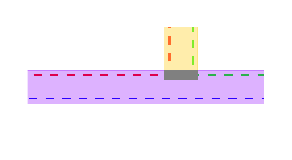
\begin{tikzpicture}[scale=0.6]
		\clip (3,1.3) rectangle (8,3.5);
		% clusters
		\draw[thick,dashed,red] (0,5) -- (0,2.5) -- (6,2.5) -- (6,5);
		\draw[thick,dashed,green] (6.5,5) -- (6.5,2.5) -- (12.5,2.5) -- (12.5,5);
		\draw[thick,dashed,red] (0,-5) -- (0,-2.5) -- (6,-2.5) -- (6,-5);
		\draw[thick,dashed,red] (6.5,-5) -- (6.5,-2.5) -- (12.5,-2.5) -- (12.5,-5);
		
		%         % blue blocks
		\draw[thin,dashed,blue] (0,-2) rectangle ++ (10,4);
		
		
		%         % left & right chip border
		\draw[black] (-0.3,-5) -- (-0.3,5);
		\draw[black] (12.8,-5) -- (12.8,5);
		
		
		
		%         % blockages in T shaped gaps
		
	
		
		
		
		{	
			\draw[customviolet,fill, opacity=0.3] (-0.3,1.9) rectangle (12.8,2.6);
			\draw[customviolet,fill, opacity=0.3] (-0.3,-1.9) rectangle (12.8,-2.6);
		}
		
	{	
		
		
			\draw[mustardyellow,fill, opacity=0.5] (12.4,2.4) rectangle (12.8,5);
		
			
		
			\draw[mustardyellow,fill, opacity=0.5] (5.9,2.4) rectangle (6.6,5);
		
		
			\draw[gray,fill] (12.4,2.6) rectangle (12.8,2.4);
			\draw[gray,fill] (4.9,-1.9) rectangle (5.6,-2.1);
			\draw[gray,fill] (9.9,-1.9) rectangle (10.6,-2.1);
			\draw[gray,fill] (12.4,-1.9) rectangle (12.8,-2.1);
			\draw[gray,fill] (12.4,-2.4) rectangle (12.8,-2.6);
			\draw[gray,fill] (5.9,2.4) rectangle (6.6,2.6);
			\draw[gray,fill] (5.9,-2.4) rectangle (6.6,-2.6);
			
			
		}

	
		%%%%%TODO copy to reuse conts
		
		
		%%%%%%%%%%%% T-junction thingies
	
	\end{tikzpicture}
\raggedright
{\footnotesize \begin{spacing}{0.9}
	 Blockage structure on T-junction of corridors. Blockages on layers with horizontal/vertical prefered direction are purple/yellow, completely blocked areas are gray.\end{spacing}	}

\end{minipage}
  % insert picture here
  
  In addition, we modify the tile structure of global routing to have a guaranteed
  tile border on every block border and where the border blockages end. This way the router
  cannot introduce vias in the tiles adjacent bock borders and  track assignment can assign the short segments crossing the block border.
  The global router has to  support non-uniform tiles.
  
 
  Also track assignment assigns segments passing through both borders.
  
  
  %TODO maybe pins in different directions, different sizes for different wiretypes?	
 		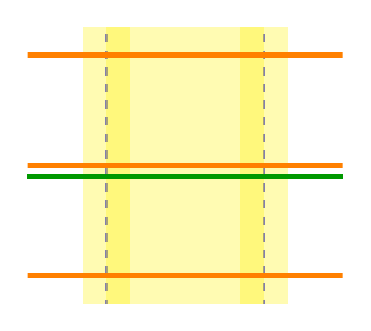
\begin{tikzpicture}[yscale=0.7]
 			
 			% Parameters
 			\def\nrows{4}
 			\def\ncols{3}
 			\def\rowheight{2.0}
 			\def\colwidth{2.0}
 			\def\bbwidth{0.3}
 			\clip (1, -\nrows*\rowheight + 1.5) rectangle (\ncols*\colwidth-1, -1.5);
 			
 			%	\foreach \i in {0,...,\nrows} {
 				%		\ifodd\i
 				%		\fill[gray!20] (0,-\i*\rowheight) rectangle (\ncols*\colwidth,-\i*\rowheight+\rowheight);
 				%		\else
 				%		\fill[gray!30] (0,-\i*\rowheight) rectangle (\ncols*\colwidth,-\i*\rowheight+\rowheight);
 				%		\fi
 				%	}
 			
 			% block borders
 			\foreach \j in {1,...,\numexpr\ncols-1\relax} {
 				\draw[blue!70, dashed,thick] (\j*\colwidth, \rowheight) -- (\j*\colwidth,-\nrows*\rowheight);
 			}
 			
 			% border blockage
 			\foreach \j in {1,...,\numexpr\ncols-1\relax} {
 				\fill[yellow, opacity=0.3]
 				(\colwidth*\j - \bbwidth, \rowheight) rectangle (\colwidth*\j + \bbwidth, -\nrows*\rowheight);
 			}
 			
 			% Fill gap
 			\fill[yellow, opacity=0.3]
 			(\colwidth*1, \rowheight) rectangle (\colwidth*2, -\nrows*\rowheight);
 			
 			
 			% track borders
 			\foreach \i in {0,...,\numexpr\nrows-1\relax} {
 				\draw[orange,line width=2pt ] (0,-\i*\rowheight) -- (\ncols*\colwidth,-\i*\rowheight);
 			}
 			
 			% Wire segments right, left block
 			\foreach \y in {-1.6,-2.0,-2.2,-2.4,-2.6,-3.2} {
 				\draw[green!60!black,line width=2pt] (0,-4.2) -- (1.3  ,-4.2);
 				\draw[green!60!black,line width=2pt] ((\ncols*\colwidth -1.3,-4.2) -- (\ncols*\colwidth ,-4.2);
 			}
 			
 			
 			% route before TA
 			\foreach \y in {-1.8,-2.0,-2.2,-2.4,-2.6,-3.2} {
 				\draw[green!60!black,line width=2pt] (0 + 0.2*\colwidth,-4.2) -- (\ncols*\colwidth ,-4.2);
 			}
 			% route after TA
 			\foreach \y in {-1.8,-2.2,-2.4,-2.6,-3.2,-4.6,-4.8,-5.6} {
 				%\draw[green!60!black,line width=2pt, opacity=0.3] (0 + 0.2*\colwidth,\y) -- (\ncols*\colwidth ,\y);
 			}	
 			
 			% extract pin postions (take y positions from after TA)
 			\def\pinwidth{0.15}
 			
 			%    \foreach \y in {-1.8,-2.2,-2.4,-2.6,-3.2,-4.6,-4.8,-5.6,} {
 				%    	\draw[thick] (0, \y) -- (\colwidth*3, \y);
 				%    	 \begin{scope}[shift={(\colwidth*2+\pinwidth, \y)}]		
 					%    		\filldraw[fill=black] (-0.15, 0) -- (-0.25, 0.1) -- (-0.25, -0.1) -- cycle;
 					%    		\filldraw[fill=white, draw=black] (-0.15, -0.1) rectangle (0.15, 0.1);
 					%    	\end{scope}
 				%    
 				%    	
 				%    
 				%     	\begin{scope}[shift={(\colwidth-\pinwidth, \y)}]		
 					%    		\filldraw[fill=black] (-0.15, 0) -- (-0.25, 0.1) -- (-0.25, -0.1) -- cycle;
 					%    		\filldraw[fill=white, draw=black] (-0.15, -0.1) rectangle (0.15, 0.1);
 					%    	\end{scope}  	
 				%    }	
 			
 			
 			
 			
 			
 		\end{tikzpicture} 
 	\hfill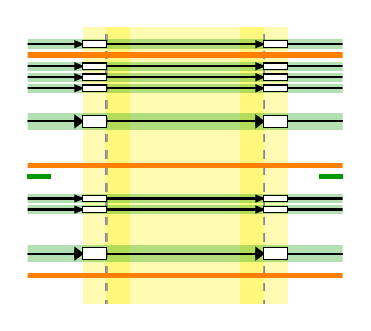
\begin{tikzpicture}[yscale=0.7]
 			
 			% Parameters
 			\def\nrows{4}
 			\def\ncols{3}
 			\def\rowheight{2.0}
 			\def\colwidth{2.0}
 			\def\bbwidth{0.3}
 			\clip (1, -\nrows*\rowheight + 1.5) rectangle (\ncols*\colwidth-1, -1.5);
 			
 			%	\foreach \i in {0,...,\nrows} {
 				%		\ifodd\i
 				%		\fill[gray!20] (0,-\i*\rowheight) rectangle (\ncols*\colwidth,-\i*\rowheight+\rowheight);
 				%		\else
 				%		\fill[gray!30] (0,-\i*\rowheight) rectangle (\ncols*\colwidth,-\i*\rowheight+\rowheight);
 				%		\fi
 				%	}
 			
 			% block borders
 			\foreach \j in {1,...,\numexpr\ncols-1\relax} {
 				\draw[blue!70, dashed,thick] (\j*\colwidth, \rowheight) -- (\j*\colwidth,-\nrows*\rowheight);
 			}
 			
 			% border blockage
 			\foreach \j in {1,...,\numexpr\ncols-1\relax} {
 				\fill[yellow, opacity=0.3]
 				(\colwidth*\j - \bbwidth, \rowheight) rectangle (\colwidth*\j + \bbwidth, -\nrows*\rowheight);
 			}
 			
 			% Fill gap
 			\fill[yellow, opacity=0.3]
 			(\colwidth*1, \rowheight) rectangle (\colwidth*2, -\nrows*\rowheight);
 			
 			
 			% track borders
 			\foreach \i in {0,...,\numexpr\nrows-1\relax} {
 				\draw[orange,line width=2pt ] (0,-\i*\rowheight) -- (\ncols*\colwidth,-\i*\rowheight);
 			}
 			
 			% Wire segments right, left block
 			\foreach \y in {-1.6,-2.0,-2.2,-2.4,-2.6,-3.2} {
 				\draw[green!60!black,line width=2pt] (0,-4.2) -- (1.3  ,-4.2);
 				\draw[green!60!black,line width=2pt] (\ncols*\colwidth -1.3,-4.2) -- (\ncols*\colwidth ,-4.2);
 			}
 			
 			
 			% route before TA
 			\foreach \y in {-1.8,-2.0,-2.2,-2.4,-2.6,-3.2} {
 				%\draw[green!60!black,line width=2pt] (0 + 0.2*\colwidth,-4.2) -- (\ncols*\colwidth ,-4.2);
 			}
 			% route after TA
 			\foreach \y in {-1.8,-2.2,-2.4,-2.6,-4.6,-4.8} {
 				\draw[green!60!black,line width=0.12cm, opacity=0.3] (0 + 0.2*\colwidth,\y) -- (\ncols*\colwidth ,\y);
 			}	
 			\foreach \y in {-3.2,-5.6} {
 				\draw[green!60!black,line width=0.22cm, opacity=0.3] (0 + 0.2*\colwidth,\y) -- (\ncols*\colwidth ,\y);
 			}	
 			
 			% extract pin postions (take y positions from after TA)
 			\def\pinwidth{0.15}
 			
 			
 			
 			\foreach \y in {-1.8,-2.2,-2.4,-2.6,-3.2,-4.6,-4.8,-5.6,} {
 				\draw[thick] (0, \y) -- (\colwidth*3, \y);
 				\begin{scope}[shift={(\colwidth*2+\pinwidth, \y)}]		
 					\filldraw[fill=black] (-0.15, 0) -- (-0.25, 0.06) -- (-0.25, -0.06) -- cycle;
 					\filldraw[fill=white, draw=black] (-0.15, -0.06) rectangle (0.15, 0.06);
 				\end{scope}
 				
 				
 				
 				\begin{scope}[shift={(\colwidth-\pinwidth, \y)}]		
 					\filldraw[fill=black] (-0.15, 0) -- (-0.25, 0.06) -- (-0.25, -0.06) -- cycle;
 					\filldraw[fill=white, draw=black] (-0.15, -0.06) rectangle (0.15, 0.06);
 				\end{scope}  	
 			}
 			\foreach \y in {-3.2,-5.6,} {
 				\draw[thick] (0, \y) -- (\colwidth*3, \y);
 				\begin{scope}[shift={(\colwidth*2+\pinwidth, \y)}]		
 					\filldraw[fill=black] (-0.15, 0) -- (-0.25, 0.11) -- (-0.25, -0.11) -- cycle;
 					\filldraw[fill=white, draw=black] (-0.15, -0.11) rectangle (0.15, 0.11);
 				\end{scope}
 				
 				
 				
 				\begin{scope}[shift={(\colwidth-\pinwidth, \y)}]		
 					\filldraw[fill=black] (-0.15, 0) -- (-0.25, 0.11) -- (-0.25, -0.11) -- cycle;
 					\filldraw[fill=white, draw=black] (-0.15, -0.11) rectangle (0.15, 0.11);
 				\end{scope}  	
 			}		
 			
 		\end{tikzpicture} 
 {\footnotesize \begin{spacing}{0.9}
 		Left: global routing solution respecting border and fill gap obstacles, allowing only horizontal routing
 		Right: pins are added according to wireshapes after track assignment (run only in corridor region)
 		The dashed blue lines are the block borders, in yellow are the border blockages that block vertical layers.
 	\end{spacing}	}
 
 	
	\blockbreak
	\textbf{Routing Topologies}
	Our way to generate routing topologies ensures:
	\begin{itemize}
		\item Reuse blocks are entered only once for connecting to the sinks inside (further entries for connections going through them are possible)
		\item If no port assignment is given, then the length of any source-sink path through the topology
		should be within a factor $(1+\epsilon)$ of the source-sink distance, (usually $\epsilon=.1$)
		\item If a (partial) port assignment is given, terminals in blocks with assigned pins are connected over the assigned pin positions.
	\end{itemize}
	We use a two step Steiner tree oracle for the nets in  global routing.
	First, we compute a 2D obstacle-avoiding Steiner tree topology  that is then embedded into the 3D global routing graph.
	
	
	For the topology  we aim  for an approximate shortest path topology w.r.t. obstacles. The length of any source-sink path through the topology
	should be within a factor $(1+\epsilon)$ of the source-sink distance, usually $\epsilon=.1$ 
	Later the embedding into the global routing graph considers the congestion prices and sink delay prices provided by the resource sharing algorithm (see \cite{BRGTiming2}).
	It is allowed to  introduce detours to avoid congestion and it decides the  layers and wire configuration that greatly determine the signal speed and routing congestion.
	
	Here, we describe how we compute hierarchical topologies with the aim to avoid too many pins.
	Given  a net with root $r$ and terminal sink set $S$ we want to find a geometric Steiner topology $Y$ s.t.
	the paths in $Y$ from $r$ to each $s\in S$  are  approximate shortest paths and $Y$ enters each block at most once.
	
	First, we cluster the sinks $S = S_1\cdot{\cup}\dots\cdot{\cup} S_n$ by the containing block and add a new cluster root $v_i$ for each non-empty cluster $S_i \neq\emptyset$ ($i\in [k]$).
	We place  $v_i$ at  the projection of the root onto the bounding box of $S_i$. 
	In the reuse setting (see Section~\ref{sec:reuse}), we might be given a partial pin assignment, i.e. predefined input pin positions for some blocks. %TODO {Das muss spaeter noch besser beschrieben werden}
	
	
	Now, we compute a  blockage-avoiding approximate geometric shortest path $r$-arborescence $Y_{top}$ with the cluster roots as sinks.
	To this end we compute a shallow-light arborescence \cite{ShallowLight} with distances as delay bounds.
	It is carried out in a  blockage-avoiding visibility graph that supports blockages with direction restrictions from Section~\ref{sec:tiles_n_border_blockages}.
	A blockage with vertical/horizontal direction restriction may be traversed vertically/horizontally (see \cite{bihler-dissertation} for details).
	
	Now we traverse the vertices $v\in V(Y_{top})$ in reverse topological order.
	Let $B_i$ be the block in which $v$ is placed and $V_i\ni v$ be the vertices in the maximal connected component of $Y_{top}$ induced by vertices placed inside $B_i$.
	Whenever the parent of $v$ is placed in a different block than $v$, we compute an approximate shortest path $v$-arborescence for the  sinks in $S_i \cup \Gamma_{Y_{top}}^+(V_i)$,
	where $\Gamma_{Y_{top}}^+(V_i)$ denotes the successors in other blocks.
	$Y$ is the union of all these arborescences. The following Theorem is easy to see.\\
	
	The embedding into the 3D global routing graph traverses the vertices $v\in V(Y)$  bottom-up and embeds sibling paths $\delta^+(v)$
	until they meet near the position of $v$ (see \cite{BRGTiming2}).
	Crossing  block boundaies is only allowed in the direction of the target $v$.
	In case of rectangular blocks this avoids zig-zagging along block borders.\\
\end{blockrow}
 \begin{blockrow}
 	
\blocktitle{Multiply Instantiated Reuse Blocks}
\begin{minipage}{0.6\blockwidth}
Equivalent reuse blocks (blue) can be mirrored on the x- and y- axis with respect to each other (indicated by {\sffamily F}).
We assume that we are given an equivalence relation on the terminals in different blocks $B_i$ ($i\in [k]$), with equivalent terminals being at equivalent positions relative to their blocks.

If two terminals  in block $B_i$ are part of a inter-block net $N$, their equivalent terminals in another block must be connected
to a common net or must both be floating (unconnected). In the following we call a terminal \textit{floating}, if it is not connected to a net
but equivalent to a terminal in a inter-block net. 
%
We need to achieve pin positions at the same relative border positions and equivalent pin graphs on the  reuse blocks $B_1,...,B_k$, to be able to use the same routing for all reuse blocks.

We compute pin positions (or more precisely pin graph parts) on one arbitrarily chosen reuse block $B_1$ that we call the \textit{leader} (solid line). 
Then, we  force these positions on the other reuse blocks $B_1\dots, B_k$, called the \textit{followers} (dashed lines). 
For that to work correctly, we need to consider two things: 

	
	
\end{minipage}
\begin{minipage}{0.3\blockwidth}
	\centering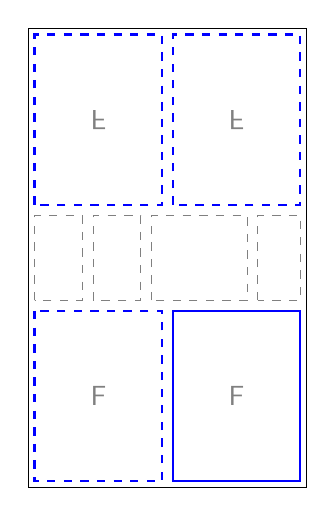
\begin{tikzpicture}[scale=0.27]
	\draw[thick,dashed,blue] (0,2.5) rectangle ++ (6,8);
	\draw[thick,dashed,blue] (6.5,2.5) rectangle ++ (6,8);
	\draw[thick,dashed,blue] (0,-2.5) rectangle ++ (6,-8);
	\draw[thick,blue] (6.5,-2.5) rectangle ++ (6,-8);
	\node[yscale=-1] at (3, 6.5) { \textcolor{gray}{{\sffamily F}}};
	\node[yscale=-1] at (9.5, 6.5) { \textcolor{gray}{{\sffamily F}}};
	\node at (3, -6.5) { \textcolor{gray}{{\sffamily F}}};
	\node at (9.5, -6.5) { \textcolor{gray}{{\sffamily F}}};
	
	\draw[thin,dashed,gray] (0,-2) rectangle ++ (2.25,4);
	\draw[thin,dashed,gray] (2.75,-2) rectangle ++ (2.25,4);
	\draw[thin,dashed,gray] (5.5,-2) rectangle ++ (4.5,4);
	\draw[thin,dashed,gray] (10.5,-2) rectangle ++ (2,4);
	
	\draw[black] (-0.3,-10.8) rectangle ++ (0.6+6+0.5+6, 0.6+8+8+4+1);
\end{tikzpicture}
\end{minipage}\\

\begin{enumerate}
%TODO make this shorter
\item[\raisebox{2.3cm}{1.}] \begin{minipage}{0.5\blockwidth}
	
Pin positions that are good  for the leader might cause huge detours or, due to obstacles around the block borders, even be infeasible for the followers.
We align the blockage structure around the reuse blocks by adding a copy of every blockage within the border region of the reuse blocks to the equivalent positions around the other reuse blocks. With these extra reuse blockages (orange)  we ensure feasibility. Pin intervals ensure that pin positions lie, if possible, on a shortest source sink path.
\end{minipage}
\hfill
\begin{minipage}{0.4\blockwidth}
	\centering
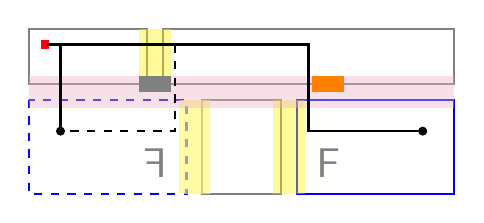
\begin{tikzpicture}
	% Parameters
	\def\nrows{4}
	\def\ncols{3}
	\def\rowheightu{0.7}
	\def\rowheightl{1.2}
	\def\corridorwidth{0.2}
	\def\reusewidth{2.0}
	\def\otherwidth{1.0}
	\def\uppersmallwidth{1.5}
	\def\sinkscale{0.3}
	\def\rootscale{0.4}
	
	%pins
	\node[draw=red, fill=red, rectangle,scale=\rootscale] (r1) at (0.2,0.7) {};
	\node[shape=circle, draw=black, fill=black, scale=\sinkscale] (s1) at (0.4,-0.4) {};
	\node[shape=circle, draw=black, fill=black, scale=\sinkscale] (s11) at (2*\reusewidth+2*\corridorwidth+ \otherwidth-0.4,-0.4) {};
	\node[color=gray, thick, scale=1.5, xscale=1] at (\reusewidth+2*\corridorwidth +\otherwidth+0.4,-\rowheightl +0.4) {{\sffamily F}};

	{{\sffamily F}};

	\node[color=gray, thick, scale=1.5,xscale=-1] at (\reusewidth-0.4,-\rowheightl +0.4) {{\sffamily F}};
	
	%blocks
	\draw[thick,blue,dashed] (0,0) rectangle (\reusewidth,0-\rowheightl);
	\draw[thick,gray] (\reusewidth+\corridorwidth,0) rectangle(\reusewidth+\corridorwidth+\otherwidth,0-\rowheightl);
	\draw[thick,blue] (2*\reusewidth+2*\corridorwidth +\otherwidth,0) rectangle(\reusewidth+2*\corridorwidth+\otherwidth,0-\rowheightl);
	\draw[thick,gray] (2*\reusewidth+2*\corridorwidth +\otherwidth,\corridorwidth) rectangle(\corridorwidth +\uppersmallwidth,\corridorwidth+\rowheightu);
	\draw[thick,gray] (\uppersmallwidth,\corridorwidth) rectangle(0,\corridorwidth+\rowheightu);
	
	%nets
	%\draw[dashed, gray] (r1)--(s1);
	%\draw[dashed, gray] (r1)--(s11);
	%\draw[dashed, gray] (r2)--(s2);
	%\draw[dashed, gray] (r3)--(s3);
	
	%blockages
	\fill[yellow, opacity=0.4]
	(\reusewidth - 0.1, 0-\rowheightl) rectangle (\reusewidth + 0.1 + \corridorwidth, 0);
	\fill[yellow, opacity=0.4] (\reusewidth + \corridorwidth +\otherwidth- 0.1, 0-\rowheightl) rectangle (\reusewidth +\otherwidth+ 0.1 + 2*\corridorwidth, 0);
	\fill[yellow!30, opacity=0.4]
	(\reusewidth - 0.1, 0-\rowheightl) rectangle (\reusewidth + 0.1 + \corridorwidth, 0);
	\fill[purple!30, opacity=0.4] (0, 0-0.1) rectangle (2*\reusewidth +\otherwidth + 2*\corridorwidth, 0+\corridorwidth+0.1);
	\fill[yellow, opacity=0.4] (\uppersmallwidth- 0.1, \corridorwidth) rectangle (\corridorwidth +\uppersmallwidth+ 0.1, \corridorwidth+\rowheightu);
	\fill[gray] (\uppersmallwidth-0.1, \corridorwidth+0.1) rectangle (\uppersmallwidth+0.1+\corridorwidth, \corridorwidth-0.1);
	\fill[orange] (2*\reusewidth+2*\corridorwidth +\otherwidth-\uppersmallwidth+0.1, \corridorwidth+0.1) rectangle (2*\reusewidth+\corridorwidth +\otherwidth-\uppersmallwidth-0.1, \corridorwidth-0.1);
	
	

	
	%Routing pass 1 no pis
	\node[] (r1) at (0.1,0.7) {};
	\draw [thick] (r1)--(0.4, 0.7) --(s1);
	\draw [thick] (r1) -- (3.55, 0.7) -- (3.55, -0.4)--(s11);
	\draw [thick, dashed] (1.85,0.7) -- (1.85, -0.4) --(s1);
	
	


	
	
	
	
	
	
\end{tikzpicture}	
\raggedright
{\footnotesize \begin{spacing}{0.9}
		Possible routing without reuse blocks. When the pin position of this routing from the leader is forced on the follower, a huge detour is caused(dashed).\end{spacing}	}
\end{minipage}
%When the pins of a net $N_i$ inside $B_i$ are at the same relative positions as the pins of a net $N_j$ inside $B_j$, the respective pin graph parts have to be the same and we say that $(N_j,B_j)\sim (N_j,B_j)$ inducing an an equivalence relation on net-block combinations.
%When the pin positions of the \textit{leader} are forced onto the followers an ideal pin position for the net $N_1$ in the leader $B_1$ could cause huge detours for one of the corresponding net-block combinations $(N_j,B_j)\in [(N_1,B_1)]$ in the followers (see \ref{figure}). Even worse, the pin position on the leader could even be infeasible for the follower. Our way to avoid such situations that are pin intervals (\ref{PIsection}) and additional reuse way to copy blockages \ref{reuseblockagessection}. %Maybe refer to figure

\item [{2.}] Floating terminals  must be connected to pins and create pins  for \textit{feedthroughs}, i.e.\
nets that are routed through reuse blocks, without connecting to anything inside them. 
Floating terminals and feedthroughs might be different in each reuse block, but finally, they must be implemented by all reuse blocks. To this end, virtual nets representing such feedthroughs
or connections to floating terminals are added to the leader, and then those followers where they are not represented already.
\end{enumerate}
%TODO is this said else where? we allow only one entry or exit for connecting the terminals to the root, or the signal from the root leaving the block. Therefore there is at most one pin for each net-block-combination... 
%TODO say that connections between them are forbidden
%TODO somewhere say which that feedthrough sinks might not connect to something, but feedthrough sources always need to be served 
% TODO cite fine
\textbf{Pin Intervals:}
We ensure to find pin positions that are good for every equivalent block and visible in the first routing pass as follows:
We predefine pin intervals at the block borders, that the router is forced to route through.
We first choose an interval (often just a point) on the boundary such that the worst detour w.r.t. the  $\ell_1$-metric among all equivalent blocks in an individual net routing is minimized.
This interval is then increased  by a constant value to give the router flexibility in avoiding congestion.

We usually allow only a single pin to serve the sinks or source in a block.
For each block border, we use elementary geometry to compute the minimum detour pin interval w.r.t. all blocks on that border.  If blockages prevent
routing through that interval we try the positions at both ends of the
blockage.  Finally, we take the best interval over all borders.

To align routing in the first pass we will shrink large intervals to an interval of maximum  length $\delta>0$.
Similarly, to improve routability we will expand small intervals to a minimum length $\delta$.

In principle, it could be preferable to allow $k>1$ pins position  per net, e.g. if a root in side a reuse block
has sinks north and south of a block.
If the net connects to sinks inside a reuse block, multiple pin positions, could still be interesting but would
require to add a multiplexer between pins and sinks in each block.

In this case choosing the best pin positions becomes a kind of facility location problem on the boundary.
The external sinks/sources are connected through one of the pins/facilities.


\blockbreak
\blocktitle{Flow}
The overall flow to achieve compatible pin positions is shown in Algorithm \ref{alg:reuse-alg}.
We use 3 global routing passes, each with a different purpose, and some preprocessing before each routing pass:
%TODO is it feedthrough or feethrough???
\begin{algorithm}[H] 
	\begin{enumerate}
		\item add in blockages and reuse blockages \label{step:add-blockages}
		\item choose pin intervals  \label{PIstep}
		\item \textbf{first routing pass w/o track assignment} \label{step:pass1}
		% TODO Similarly, add virtual nets connecting floating terminals with the boundary.
	%	Pin positions are bound to an interval around the computed routing position.\label{step:create-artificial-feedthroughs} \textcolor{red}{SH: rephrase this step.}
		\item Add virtual nets between artificial pins representing feedthroughs to reuse blocks \label{step:create-artificial-feedthroughs}
		\item delete pin assignment outside of reuse blocks, relax pin positions to intervals \label{step:relaxpositions}
		\item \textbf{second routing pass w/ track assignment}
		\item copy pins assignments from the leader to its followers \label{step:copy-pin-assignment}
		\item delete pin assignment outside reuse blocks
		\item \textbf{third routing pass w/ track assignment}
	\end{enumerate} % TODO: fix order , always first delete, then force to others
	\caption{Pin Assignment With Reuse Blocks.}
	\label{alg:reuse-alg}
\end{algorithm}
\begin{tabular}{cc}
	\begin{minipage}{0.5\blockwidth}
	

		  Steps~\ref{step:add-blockages} and \ref{PIstep} ensure that reuse blocks have the same set of feasible positions and use pin intervals imposing  similar and good  positions the first routing pass, which is needed to determine the feedthroughs through reuse blocks
		   	\end{minipage}    &\begin{minipage}{0.49\blockwidth}
		  \centering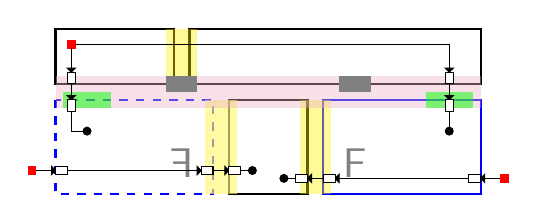
\begin{tikzpicture}
	% Parameters
	\def\nrows{4}
	\def\ncols{3}
	\def\rowheightu{0.7}
	\def\rowheightl{1.2}
	\def\corridorwidth{0.2}
	\def\reusewidth{2.0}
	\def\otherwidth{1.0}
	\def\uppersmallwidth{1.5}
	\def\sinkscale{0.3}
	\def\rootscale{0.4}
	
	%pins
	\node[draw=red, fill=red, rectangle,scale=\rootscale] (r1) at (0.2,0.7) {};
	\node[shape=circle, draw=black, fill=black, scale=\sinkscale] (s1) at (0.4,-0.4) {};
	\node[shape=circle, draw=black, fill=black, scale=\sinkscale] (s11) at (2*\reusewidth+2*\corridorwidth+ \otherwidth-0.4,-0.4) {};
	\node[color=gray, thick, scale=1.5, xscale=1] at (\reusewidth+2*\corridorwidth +\otherwidth+0.4,-\rowheightl +0.4) {{\sffamily F}};
	\node[shape=circle, draw=black, fill=black, scale=\sinkscale] (s2) at (\reusewidth+\corridorwidth +0.3,-0.9) {};
	\node[shape=circle, draw=black, fill=black, scale=\sinkscale] (s3) at (\reusewidth+\corridorwidth +0.7,-1) {};
	\node[draw=red, fill=red, rectangle,scale=\rootscale] (r2) at (-0.3,-0.9) {};
	{{\sffamily F}};
	\node[draw=red, fill=red, rectangle,scale=\rootscale] (r3) at (2*\reusewidth+2*\corridorwidth +\otherwidth+0.3,-1) {};
	\node[color=gray, thick, scale=1.5,xscale=-1] at (\reusewidth-0.4,-\rowheightl +0.4) {{\sffamily F}};
	
	%blocks
		\draw[thick,blue,dashed] (0,0) rectangle (\reusewidth,0-\rowheightl);
	\draw[thick] (\reusewidth+\corridorwidth,0) rectangle(\reusewidth+\corridorwidth+\otherwidth,0-\rowheightl);
	\draw[thick,blue] (2*\reusewidth+2*\corridorwidth +\otherwidth,0) rectangle(\reusewidth+2*\corridorwidth+\otherwidth,0-\rowheightl);
	\draw[thick] (2*\reusewidth+2*\corridorwidth +\otherwidth,\corridorwidth) rectangle(\corridorwidth +\uppersmallwidth,\corridorwidth+\rowheightu);
	\draw[thick] (\uppersmallwidth,\corridorwidth) rectangle(0,\corridorwidth+\rowheightu);
	
	%nets
	%\draw[dashed, gray] (r1)--(s1);
	%\draw[dashed, gray] (r1)--(s11);
	%\draw[dashed, gray] (r2)--(s2);
	%\draw[dashed, gray] (r3)--(s3);
	
	%blockages
	\fill[yellow, opacity=0.4]
	(\reusewidth - 0.1, 0-\rowheightl) rectangle (\reusewidth + 0.1 + \corridorwidth, 0);
	\fill[yellow, opacity=0.4] (\reusewidth + \corridorwidth +\otherwidth- 0.1, 0-\rowheightl) rectangle (\reusewidth +\otherwidth+ 0.1 + 2*\corridorwidth, 0);
	\fill[yellow!30, opacity=0.4]
	(\reusewidth - 0.1, 0-\rowheightl) rectangle (\reusewidth + 0.1 + \corridorwidth, 0);
	\fill[purple!30, opacity=0.4] (0, 0-0.1) rectangle (2*\reusewidth +\otherwidth + 2*\corridorwidth, 0+\corridorwidth+0.1);
	\fill[yellow, opacity=0.4] (\uppersmallwidth- 0.1, \corridorwidth) rectangle (\corridorwidth +\uppersmallwidth+ 0.1, \corridorwidth+\rowheightu);
	\fill[gray] (\uppersmallwidth-0.1, \corridorwidth+0.1) rectangle (\uppersmallwidth+0.1+\corridorwidth, \corridorwidth-0.1);
	\fill[gray] (2*\reusewidth+2*\corridorwidth +\otherwidth-\uppersmallwidth+0.1, \corridorwidth+0.1) rectangle (2*\reusewidth+\corridorwidth +\otherwidth-\uppersmallwidth-0.1, \corridorwidth-0.1);
	
	%pin intervals
	\fill[green, opacity=0.5] (2*\reusewidth+2*\corridorwidth+ \otherwidth-0.1, -0.1) rectangle (2*\reusewidth+2*\corridorwidth+ \otherwidth-0.7, 0.1);
	\fill[green, opacity=0.5] (0.1, -0.1) rectangle (0.7, 0.1);
	
	%Routing pass 1
	\def\xppi{0.2}
	\def\xppii{2*\reusewidth+2*\corridorwidth +\otherwidth-0.4}
	\def\yppi{-0.9}
	\def\yppii{-1}
	\def\ps{0.075}
	\draw (r2)--(s2);
	\draw (r3)--(s3);
	\draw (r1)--(\xppi, -0.4) --(s1);
	\draw (r1) -- (\xppii, 0.7) -- (\xppii, -0.4)--(s11);
	
	
	%Pins routing pass 1
	\foreach \x in {\xppi,\xppii} {            	
		\begin{scope}[shift={(\x, -\ps)},rotate=-90, scale=0.5]		
			\filldraw[fill=black] (-0.15, 0) -- (-0.25, 0.1) -- (-0.25, -0.1) -- cycle;
			\filldraw[fill=white, draw=black] (-0.15, -0.1) rectangle (0.15, 0.1);
		\end{scope}		
		
		\begin{scope}[shift={(\x, \corridorwidth+\ps)},rotate=-90, scale=0.5]		
			\filldraw[fill=black] (-0.15, 0) -- (-0.25, 0.1) -- (-0.25, -0.1) -- cycle;
			\filldraw[fill=white, draw=black] (-0.15, -0.1) rectangle (0.15, 0.1);
		\end{scope}		               	
	}
	
	\foreach \x in {0+\ps,\reusewidth-\ps,\reusewidth+\corridorwidth+\ps} {            	
		\begin{scope}[shift={(\x, \yppi)}, scale=0.5]		
			\filldraw[fill=black] (-0.15, 0) -- (-0.25, 0.1) -- (-0.25, -0.1) -- cycle;
			\filldraw[fill=white, draw=black] (-0.15, -0.1) rectangle (0.15, 0.1);
		\end{scope}		             	
	}
	\foreach \x in {\reusewidth+\corridorwidth+\otherwidth-\ps,\reusewidth+2*\corridorwidth+\otherwidth+\ps,2*\reusewidth+2*\corridorwidth+\otherwidth-\ps} {            	
		\begin{scope}[shift={(\x, \yppii)}, scale=0.5,rotate=180]		
			\filldraw[fill=black] (-0.15, 0) -- (-0.25, 0.1) -- (-0.25, -0.1) -- cycle;
			\filldraw[fill=white, draw=black] (-0.15, -0.1) rectangle (0.15, 0.1);
		\end{scope}		             	
	}
	
	
	
	
	
	
\end{tikzpicture}\end{minipage}\\
\multicolumn{2}{c}{} \\
\begin{minipage}{0.5\blockwidth}
In step \ref{step:create-artificial-feedthroughs} we create for each feedthrough through a reuse block an artificial net with artificial pins on the boundary of each equivalent block. The positions of the artificial pins in the leader will determine the positions of the pins of this feedthrough in the follower.
This may leave overlapping pins. Thus, we relax pin positions to intervals (step \ref{step:relaxpositions}) to give the router enough freedom to legalize the pin positions. 

\end{minipage}&\begin{minipage}{0.49\blockwidth}
\centering

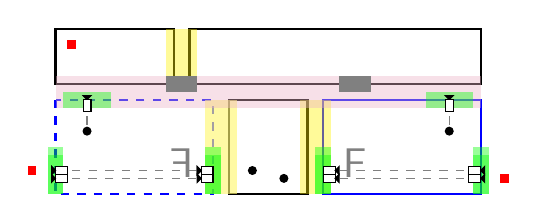
\begin{tikzpicture}
	% Parameters
	\def\nrows{4}
	\def\ncols{3}
	\def\rowheightu{0.7}
	\def\rowheightl{1.2}
	\def\corridorwidth{0.2}
	\def\reusewidth{2.0}
	\def\otherwidth{1.0}
	\def\uppersmallwidth{1.5}
	\def\sinkscale{0.3}
	\def\rootscale{0.4}
		\def\xppi{0.4}
	\def\xppii{2*\reusewidth+2*\corridorwidth +\otherwidth-0.4}
	\def\yppi{-0.9}
	\def\yppii{-1}
	\def\ps{0.075}
	
	\draw[dashed,gray] (\xppi,0) --(0.4,-0.4);
	\draw[dashed,gray] (\xppii,0) --(2*\reusewidth+2*\corridorwidth+ \otherwidth-0.4,-0.4);
	
	%pins
	\node[draw=red, fill=red, rectangle,scale=\rootscale] (r1) at (0.2,0.7) {};
	\node[shape=circle, draw=black, fill=black, scale=\sinkscale] (s1) at (0.4,-0.4) {};
	\node[shape=circle, draw=black, fill=black, scale=\sinkscale] (s11) at (2*\reusewidth+2*\corridorwidth+ \otherwidth-0.4,-0.4) {};
	\node[color=gray, thick, scale=1.5, xscale=1] at (\reusewidth+2*\corridorwidth +\otherwidth+0.4,-\rowheightl +0.4) {{\sffamily F}};
	\node[shape=circle, draw=black, fill=black, scale=\sinkscale] (s2) at (\reusewidth+\corridorwidth +0.3,-0.9) {};
	\node[shape=circle, draw=black, fill=black, scale=\sinkscale] (s3) at (\reusewidth+\corridorwidth +0.7,-1) {};
	\node[draw=red, fill=red, rectangle,scale=\rootscale] (r2) at (-0.3,-0.9) {};
	{{\sffamily F}};
	\node[draw=red, fill=red, rectangle,scale=\rootscale] (r3) at (2*\reusewidth+2*\corridorwidth +\otherwidth+0.3,-1) {};
	\node[color=gray, thick, scale=1.5,xscale=-1] at (\reusewidth-0.4,-\rowheightl +0.4) {{\sffamily F}};
	
	%blocks
		\draw[thick,blue,dashed] (0,0) rectangle (\reusewidth,0-\rowheightl);
	\draw[thick] (\reusewidth+\corridorwidth,0) rectangle(\reusewidth+\corridorwidth+\otherwidth,0-\rowheightl);
	\draw[thick,blue] (2*\reusewidth+2*\corridorwidth +\otherwidth,0) rectangle(\reusewidth+2*\corridorwidth+\otherwidth,0-\rowheightl);
	\draw[thick] (2*\reusewidth+2*\corridorwidth +\otherwidth,\corridorwidth) rectangle(\corridorwidth +\uppersmallwidth,\corridorwidth+\rowheightu);
	\draw[thick] (\uppersmallwidth,\corridorwidth) rectangle(0,\corridorwidth+\rowheightu);
	
	%nets
	%\draw[dashed, gray] (r1)--(s1);
	%\draw[dashed, gray] (r1)--(s11);
	%\draw[dashed, gray] (r2)--(s2);
	%\draw[dashed, gray] (r3)--(s3);
	
	%blockages
	\fill[yellow, opacity=0.4]
	(\reusewidth - 0.1, 0-\rowheightl) rectangle (\reusewidth + 0.1 + \corridorwidth, 0);
	\fill[yellow, opacity=0.4] (\reusewidth + \corridorwidth +\otherwidth- 0.1, 0-\rowheightl) rectangle (\reusewidth +\otherwidth+ 0.1 + 2*\corridorwidth, 0);
	\fill[yellow!30, opacity=0.4]
	(\reusewidth - 0.1, 0-\rowheightl) rectangle (\reusewidth + 0.1 + \corridorwidth, 0);
	\fill[purple!30, opacity=0.4] (0, 0-0.1) rectangle (2*\reusewidth +\otherwidth + 2*\corridorwidth, 0+\corridorwidth+0.1);
	\fill[yellow, opacity=0.4] (\uppersmallwidth- 0.1, \corridorwidth) rectangle (\corridorwidth +\uppersmallwidth+ 0.1, \corridorwidth+\rowheightu);
	\fill[gray] (\uppersmallwidth-0.1, \corridorwidth+0.1) rectangle (\uppersmallwidth+0.1+\corridorwidth, \corridorwidth-0.1);
	\fill[gray] (2*\reusewidth+2*\corridorwidth +\otherwidth-\uppersmallwidth+0.1, \corridorwidth+0.1) rectangle (2*\reusewidth+\corridorwidth +\otherwidth-\uppersmallwidth-0.1, \corridorwidth-0.1);
	
	%pin intervals
	
	\fill[green, opacity=0.4] (2*\reusewidth+2*\corridorwidth+ \otherwidth-0.1, -0.1) rectangle (2*\reusewidth+2*\corridorwidth+ \otherwidth-0.7, 0.1);
	%\fill[green, opacity=0.4] (0, -0.1) rectangle (0.5, 0.1);
	\fill[green, opacity=0.4] (2*\reusewidth+2*\corridorwidth+ \otherwidth+0.1, -0.6) rectangle (2*\reusewidth+2*\corridorwidth+ \otherwidth-0.1, -1.2);
	\fill[green, opacity=0.4] (2*\reusewidth+2*\corridorwidth+ \otherwidth+0.1, -0.7) rectangle (2*\reusewidth+2*\corridorwidth+ \otherwidth-0.1, -1.2);
	\fill[green, opacity=0.4] (\reusewidth+2*\corridorwidth+ \otherwidth+0.1, -0.6) rectangle (\reusewidth+2*\corridorwidth+ \otherwidth-0.1, -1.2);
	\fill[green, opacity=0.4] (\reusewidth+2*\corridorwidth+ \otherwidth+0.1, -0.7) rectangle (\reusewidth+2*\corridorwidth+ \otherwidth-0.1, -1.2);
	
	\begin{scope}[xscale=-1, shift={(-2*\reusewidth-2*\corridorwidth- \otherwidth ,0)}]		
		\fill[green, opacity=0.4] (2*\reusewidth+2*\corridorwidth+ \otherwidth-0.1, -0.1) rectangle (2*\reusewidth+2*\corridorwidth+ \otherwidth-0.7, 0.1);
		%\fill[green, opacity=0.4] (0, -0.1) rectangle (0.5, 0.1);
		\fill[green, opacity=0.4] (2*\reusewidth+2*\corridorwidth+ \otherwidth+0.1, -0.6) rectangle (2*\reusewidth+2*\corridorwidth+ \otherwidth-0.1, -1.2);
		\fill[green, opacity=0.4] (2*\reusewidth+2*\corridorwidth+ \otherwidth+0.1, -0.7) rectangle (2*\reusewidth+2*\corridorwidth+ \otherwidth-0.1, -1.2);
		\fill[green, opacity=0.4] (\reusewidth+2*\corridorwidth+ \otherwidth+0.1, -0.6) rectangle (\reusewidth+2*\corridorwidth+ \otherwidth-0.1, -1.2);
		\fill[green, opacity=0.4] (\reusewidth+2*\corridorwidth+ \otherwidth+0.1, -0.7) rectangle (\reusewidth+2*\corridorwidth+ \otherwidth-0.1, -1.2);
		
		
	\end{scope}
	
	%pin intervals left
	%		\fill[green, opacity=0.4] (0, -0.1) rectangle (0.5, 0.1);
	%	 (2*\reusewidth+2*\corridorwidth+ \otherwidth-0.1, -1.2);
	%		\fill[green, opacity=0.4] (0.1, -0.6) rectangle (-0.1, -1.2);
	%		\fill[green, opacity=0.4] (\reusewidth+0.1, -0.6) rectangle (\reusewidth-0.1, -1.2);
	
	%Routing pass 1

	
	\draw [dashed,gray] (\reusewidth+2*\corridorwidth+\otherwidth,\yppii)--(2*\reusewidth+2*\corridorwidth+\otherwidth,\yppii);
	
	%pins routing pass 1
	\foreach \x in {\xppi,\xppii} {            	
		\begin{scope}[shift={(\x, -\ps)},rotate=-90, scale=0.5]		
			\filldraw[fill=black] (-0.15, 0) -- (-0.25, 0.1) -- (-0.25, -0.1) -- cycle;
			\filldraw[fill=white, draw=black] (-0.15, -0.1) rectangle (0.15, 0.1);
		\end{scope}				          	
	}
	\foreach \x in {0+\ps,\reusewidth-\ps} {            	
		\begin{scope}[shift={(\x, \yppi)}, scale=0.5]		
			\filldraw[fill=black] (-0.15, 0) -- (-0.25, 0.1) -- (-0.25, -0.1) -- cycle;
			\filldraw[fill=white, draw=black] (-0.15, -0.1) rectangle (0.15, 0.1);
		\end{scope}		             	
	}
	
	
	
	%Copy in leader of subways
	\draw [dashed,gray] (\reusewidth+2*\corridorwidth+\otherwidth,\yppi)--(2*\reusewidth+2*\corridorwidth+\otherwidth,\yppi);
	\draw [dashed,gray] (0,\yppi)--(\reusewidth,\yppi);
	\foreach \x in {\reusewidth+2*\corridorwidth+\otherwidth+\ps,2*\reusewidth+2*\corridorwidth+\otherwidth-\ps} {            	
		\begin{scope}[shift={(\x, \yppi)}, scale=0.5,rotate=180]		      				
			\filldraw[fill=white, draw=black] (-0.15, -0.1) rectangle (0.15, 0.1);
			\filldraw[fill=black] (-0.15, 0) -- (-0.25, 0.1) -- (-0.25, -0.1) -- cycle;
		\end{scope}		             	
	}            		
	
	%\draw [dashed,gray] (\reusewidth+2*\corridorwidth+\otherwidth,\yppii)--(2*\reusewidth+2*\corridorwidth+\otherwidth,\yppii);	
	\foreach \x in {\reusewidth+2*\corridorwidth+\otherwidth+\ps,2*\reusewidth+2*\corridorwidth+\otherwidth-\ps} {            	
		\begin{scope}[shift={(\x, \yppii)}, scale=0.5,rotate=180]		      				
			\filldraw[fill=white, draw=black] (-0.15, -0.1) rectangle (0.15, 0.1);
			\filldraw[fill=black] (-0.15, 0) -- (-0.25, 0.1) -- (-0.25, -0.1) -- cycle;
		\end{scope}		             	
	}  
	\begin{scope}[xscale=-1, shift={(-2*\reusewidth-2*\corridorwidth- \otherwidth ,0)}]
		%\draw [dashed,gray] (\reusewidth+2*\corridorwidth+\otherwidth,\yppi)--(2*\reusewidth+2*\corridorwidth+\otherwidth,\yppi);
		\foreach \x in {\reusewidth+2*\corridorwidth+\otherwidth+\ps,2*\reusewidth+2*\corridorwidth+\otherwidth-\ps} {            	
			\begin{scope}[shift={(\x, \yppi)}, scale=0.5,rotate=180]		      				
				\filldraw[fill=white, draw=black] (-0.15, -0.1) rectangle (0.15, 0.1);
				\filldraw[fill=black] (-0.15, 0) -- (-0.25, 0.1) -- (-0.25, -0.1) -- cycle;
			\end{scope}		             	
		}            		
		
		\draw [dashed,gray] (\reusewidth+2*\corridorwidth+\otherwidth,\yppii)--(2*\reusewidth+2*\corridorwidth+\otherwidth,\yppii);
			
		\foreach \x in {\reusewidth+2*\corridorwidth+\otherwidth+\ps,2*\reusewidth+2*\corridorwidth+\otherwidth-\ps} {            	
			\begin{scope}[shift={(\x, \yppii)}, scale=0.5,rotate=180]		      				
				\filldraw[fill=white, draw=black] (-0.15, -0.1) rectangle (0.15, 0.1);
				\filldraw[fill=black] (-0.15, 0) -- (-0.25, 0.1) -- (-0.25, -0.1) -- cycle;
			\end{scope}		             	
		}  
		
	\end{scope}          		
	
	
	% Inflated PIs
	
	
	
	
\end{tikzpicture}\end{minipage}\\
\multicolumn{2}{c}{} \\
\begin{minipage}{0.5\blockwidth}

The second routing pass with track assignment (only necessary at the borders of the leader) legalizes  the pin positions the position from the first pass without moving them too much.



\end{minipage}&\begin{minipage}{0.49\blockwidth}
\centering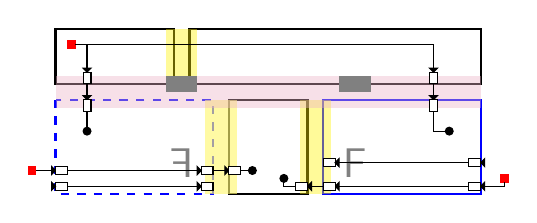
\begin{tikzpicture}
	% Parameters
	\def\nrows{4}
	\def\ncols{3}
	\def\rowheightu{0.7}
	\def\rowheightl{1.2}
	\def\corridorwidth{0.2}
	\def\reusewidth{2.0}
	\def\otherwidth{1.0}
	\def\uppersmallwidth{1.5}
	\def\sinkscale{0.3}
	\def\rootscale{0.4}
	
	%pins
	\node[draw=red, fill=red, rectangle,scale=\rootscale] (r1) at (0.2,0.7) {};
	\node[shape=circle, draw=black, fill=black, scale=\sinkscale] (s1) at (0.4,-0.4) {};
	\node[shape=circle, draw=black, fill=black, scale=\sinkscale] (s11) at (2*\reusewidth+2*\corridorwidth+ \otherwidth-0.4,-0.4) {};
	\node[color=gray, thick, scale=1.5, xscale=1] at (\reusewidth+2*\corridorwidth +\otherwidth+0.4,-\rowheightl +0.4) {{\sffamily F}};
	\node[shape=circle, draw=black, fill=black, scale=\sinkscale] (s2) at (\reusewidth+\corridorwidth +0.3,-0.9) {};
	\node[shape=circle, draw=black, fill=black, scale=\sinkscale] (s3) at (\reusewidth+\corridorwidth +0.7,-1) {};
	\node[draw=red, fill=red, rectangle,scale=\rootscale] (r2) at (-0.3,-0.9) {};
	{{\sffamily F}};
	\node[draw=red, fill=red, rectangle,scale=\rootscale] (r3) at (2*\reusewidth+2*\corridorwidth +\otherwidth+0.3,-1) {};
	\node[color=gray, thick, scale=1.5,xscale=-1] at (\reusewidth-0.4,-\rowheightl +0.4) {{\sffamily F}};
	
	%blocks
		\draw[thick,blue,dashed] (0,0) rectangle (\reusewidth,0-\rowheightl);
	\draw[thick] (\reusewidth+\corridorwidth,0) rectangle(\reusewidth+\corridorwidth+\otherwidth,0-\rowheightl);
	\draw[thick,blue] (2*\reusewidth+2*\corridorwidth +\otherwidth,0) rectangle(\reusewidth+2*\corridorwidth+\otherwidth,0-\rowheightl);
	\draw[thick] (2*\reusewidth+2*\corridorwidth +\otherwidth,\corridorwidth) rectangle(\corridorwidth +\uppersmallwidth,\corridorwidth+\rowheightu);
	\draw[thick] (\uppersmallwidth,\corridorwidth) rectangle(0,\corridorwidth+\rowheightu);
	
	%nets
	%\draw[dashed, gray] (r1)--(s1);
	%\draw[dashed, gray] (r1)--(s11);
	%\draw[dashed, gray] (r2)--(s2);
	%\draw[dashed, gray] (r3)--(s3);
	
	%blockages
	\fill[yellow, opacity=0.4]
	(\reusewidth - 0.1, 0-\rowheightl) rectangle (\reusewidth + 0.1 + \corridorwidth, 0);
	\fill[yellow, opacity=0.4] (\reusewidth + \corridorwidth +\otherwidth- 0.1, 0-\rowheightl) rectangle (\reusewidth +\otherwidth+ 0.1 + 2*\corridorwidth, 0);
	\fill[yellow!30, opacity=0.4]
	(\reusewidth - 0.1, 0-\rowheightl) rectangle (\reusewidth + 0.1 + \corridorwidth, 0);
	\fill[purple!30, opacity=0.4] (0, 0-0.1) rectangle (2*\reusewidth +\otherwidth + 2*\corridorwidth, 0+\corridorwidth+0.1);
	\fill[yellow, opacity=0.4] (\uppersmallwidth- 0.1, \corridorwidth) rectangle (\corridorwidth +\uppersmallwidth+ 0.1, \corridorwidth+\rowheightu);
	\fill[gray] (\uppersmallwidth-0.1, \corridorwidth+0.1) rectangle (\uppersmallwidth+0.1+\corridorwidth, \corridorwidth-0.1);
	\fill[gray] (2*\reusewidth+2*\corridorwidth +\otherwidth-\uppersmallwidth+0.1, \corridorwidth+0.1) rectangle (2*\reusewidth+\corridorwidth +\otherwidth-\uppersmallwidth-0.1, \corridorwidth-0.1);
	
	%Routing pass 3
	\def\xppi{0.4}
	\def\xppii{2*\reusewidth+2*\corridorwidth +\otherwidth-0.4-0.2}
	\def\yppi{-0.9}
	\def\yppii{-1.1}
	\def\ps{0.075}
	\draw (r2)--(s2);
	\draw (r3)-- (2*\reusewidth+2*\corridorwidth +\otherwidth+0.3,-1.1) --(\reusewidth+\corridorwidth +0.7,-1.1)--(s3);
	\draw (r1)--(0.4, 0.7) --(s1);
	\draw (r1) -- (\xppii, 0.7) -- (\xppii, -0.4)--(s11);
	
	
	%Pins routing pass 1
	\foreach \x in {\xppi,\xppii} {            	
		\begin{scope}[shift={(\x, -\ps)},rotate=-90, scale=0.5]		
			\filldraw[fill=black] (-0.15, 0) -- (-0.25, 0.1) -- (-0.25, -0.1) -- cycle;
			\filldraw[fill=white, draw=black] (-0.15, -0.1) rectangle (0.15, 0.1);
		\end{scope}		
		
		\begin{scope}[shift={(\x, \corridorwidth+\ps)},rotate=-90, scale=0.5]		
			\filldraw[fill=black] (-0.15, 0) -- (-0.25, 0.1) -- (-0.25, -0.1) -- cycle;
			\filldraw[fill=white, draw=black] (-0.15, -0.1) rectangle (0.15, 0.1);
		\end{scope}		               	
	}
	
	\foreach \x in {0+\ps,\reusewidth-\ps,\reusewidth+\corridorwidth+\ps} {            	
		\begin{scope}[shift={(\x, \yppi)}, scale=0.5]		
			\filldraw[fill=black] (-0.15, 0) -- (-0.25, 0.1) -- (-0.25, -0.1) -- cycle;
			\filldraw[fill=white, draw=black] (-0.15, -0.1) rectangle (0.15, 0.1);
		\end{scope}		             	
	}
	\foreach \x in {\reusewidth+\corridorwidth+\otherwidth-\ps,\reusewidth+2*\corridorwidth+\otherwidth+\ps,2*\reusewidth+2*\corridorwidth+\otherwidth-\ps} {            	
		\begin{scope}[shift={(\x, \yppii)}, scale=0.5,rotate=180]		
			\filldraw[fill=black] (-0.15, 0) -- (-0.25, 0.1) -- (-0.25, -0.1) -- cycle;
			\filldraw[fill=white, draw=black] (-0.15, -0.1) rectangle (0.15, 0.1);
		\end{scope}		             	
	}
	
	\def\yppiii{-0.8}
	\draw [] (\reusewidth+2*\corridorwidth+\otherwidth,\yppiii)--(2*\reusewidth+2*\corridorwidth+\otherwidth,\yppiii);
	\foreach \x in {\reusewidth+2*\corridorwidth+\otherwidth+\ps,2*\reusewidth+2*\corridorwidth+\otherwidth-\ps} {            	
		\begin{scope}[shift={(\x, \yppiii)}, scale=0.5,rotate=180]		      				
			\filldraw[fill=white, draw=black] (-0.15, -0.1) rectangle (0.15, 0.1);
			\filldraw[fill=black] (-0.15, 0) -- (-0.25, 0.1) -- (-0.25, -0.1) -- cycle;
		\end{scope}		             	
	}   
	
	\draw [] (0,\yppii)--(\reusewidth,\yppii);	
	\foreach \x in {0+\ps,\reusewidth-\ps} {            	
		\begin{scope}[shift={(\x, \yppii)}, scale=0.5]		      				
			\filldraw[fill=white, draw=black] (-0.15, -0.1) rectangle (0.15, 0.1);
			\filldraw[fill=black] (-0.15, 0) -- (-0.25, 0.1) -- (-0.25, -0.1) -- cycle;
		\end{scope}		             	
	}           		
	
	
	
	
	
	
	
\end{tikzpicture}\end{minipage}\\
\multicolumn{2}{c}{} \\
\begin{minipage}{0.5\blockwidth}
	Now, we enforce the legal pin positions from the leader on the followers in Step~\ref{step:copy-pin-assignment}.
	Step~\ref{step:add-blockages} guaranteed that  they are legal for the followers.
	

\end{minipage}&\begin{minipage}{0.49\blockwidth}
	\centering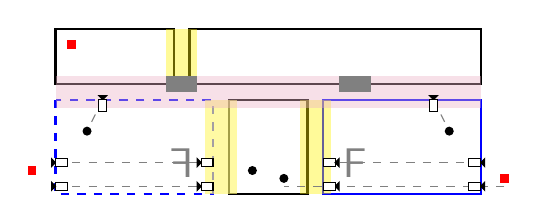
\begin{tikzpicture}
		% Parameters
		\def\nrows{4}
		\def\ncols{3}
		\def\rowheightu{0.7}
		\def\rowheightl{1.2}
		\def\corridorwidth{0.2}
		\def\reusewidth{2.0}
		\def\otherwidth{1.0}
		\def\uppersmallwidth{1.5}
		\def\sinkscale{0.3}
		\def\rootscale{0.4}
		\def\xppi{0.6}
		\def\xppii{2*\reusewidth+2*\corridorwidth +\otherwidth-0.4-0.2}
		\def\yppi{-0.8}
		\def\yppii{-1.1}
		\def\ps{0.075}
		
		\draw[dashed,gray] (\xppi,0) --(0.4,-0.4);
		\draw[dashed,gray] (\xppii,0) --(2*\reusewidth+2*\corridorwidth+ \otherwidth-0.4,-0.4);
		
		%pins
		\node[draw=red, fill=red, rectangle,scale=\rootscale] (r1) at (0.2,0.7) {};
		\node[shape=circle, draw=black, fill=black, scale=\sinkscale] (s1) at (0.4,-0.4) {};
		\node[shape=circle, draw=black, fill=black, scale=\sinkscale] (s11) at (2*\reusewidth+2*\corridorwidth+ \otherwidth-0.4,-0.4) {};
		\node[color=gray, thick, scale=1.5, xscale=1] at (\reusewidth+2*\corridorwidth +\otherwidth+0.4,-\rowheightl +0.4) {{\sffamily F}};
		\node[shape=circle, draw=black, fill=black, scale=\sinkscale] (s2) at (\reusewidth+\corridorwidth +0.3,-0.9) {};
		\node[shape=circle, draw=black, fill=black, scale=\sinkscale] (s3) at (\reusewidth+\corridorwidth +0.7,-1) {};
		\node[draw=red, fill=red, rectangle,scale=\rootscale] (r2) at (-0.3,-0.9) {};
		{{\sffamily F}};
		\node[draw=red, fill=red, rectangle,scale=\rootscale] (r3) at (2*\reusewidth+2*\corridorwidth +\otherwidth+0.3,-1) {};
		\node[color=gray, thick, scale=1.5,xscale=-1] at (\reusewidth-0.4,-\rowheightl +0.4) {{\sffamily F}};
		
		%blocks
			\draw[thick,blue,dashed] (0,0) rectangle (\reusewidth,0-\rowheightl);
		\draw[thick] (\reusewidth+\corridorwidth,0) rectangle(\reusewidth+\corridorwidth+\otherwidth,0-\rowheightl);
		\draw[thick,blue] (2*\reusewidth+2*\corridorwidth +\otherwidth,0) rectangle(\reusewidth+2*\corridorwidth+\otherwidth,0-\rowheightl);
		\draw[thick] (2*\reusewidth+2*\corridorwidth +\otherwidth,\corridorwidth) rectangle(\corridorwidth +\uppersmallwidth,\corridorwidth+\rowheightu);
		\draw[thick] (\uppersmallwidth,\corridorwidth) rectangle(0,\corridorwidth+\rowheightu);
		
		%nets
		%\draw[dashed, gray] (r1)--(s1);
		%\draw[dashed, gray] (r1)--(s11);
		%\draw[dashed, gray] (r2)--(s2);
		%\draw[dashed, gray] (r3)--(s3);
		
		%blockages
		\fill[yellow, opacity=0.4]
		(\reusewidth - 0.1, 0-\rowheightl) rectangle (\reusewidth + 0.1 + \corridorwidth, 0);
		\fill[yellow, opacity=0.4] (\reusewidth + \corridorwidth +\otherwidth- 0.1, 0-\rowheightl) rectangle (\reusewidth +\otherwidth+ 0.1 + 2*\corridorwidth, 0);
		\fill[yellow!30, opacity=0.4]
		(\reusewidth - 0.1, 0-\rowheightl) rectangle (\reusewidth + 0.1 + \corridorwidth, 0);
		\fill[purple!30, opacity=0.4] (0, 0-0.1) rectangle (2*\reusewidth +\otherwidth + 2*\corridorwidth, 0+\corridorwidth+0.1);
		\fill[yellow, opacity=0.4] (\uppersmallwidth- 0.1, \corridorwidth) rectangle (\corridorwidth +\uppersmallwidth+ 0.1, \corridorwidth+\rowheightu);
		\fill[gray] (\uppersmallwidth-0.1, \corridorwidth+0.1) rectangle (\uppersmallwidth+0.1+\corridorwidth, \corridorwidth-0.1);
		\fill[gray] (2*\reusewidth+2*\corridorwidth +\otherwidth-\uppersmallwidth+0.1, \corridorwidth+0.1) rectangle (2*\reusewidth+\corridorwidth +\otherwidth-\uppersmallwidth-0.1, \corridorwidth-0.1);
		
		%Routing pass 3
	
		\draw [dashed, gray](0,-0.8) -- (\reusewidth,-0.8);
		\draw [dashed, gray](2*\reusewidth+2*\corridorwidth +\otherwidth+0.3,-1.1) --(\reusewidth+\corridorwidth +0.7,-1.1);
		
		
		%Pins routing pass 1
		\foreach \x in {\xppi,\xppii} {            	
			\begin{scope}[shift={(\x, -\ps)},rotate=-90, scale=0.5]		
				\filldraw[fill=black] (-0.15, 0) -- (-0.25, 0.1) -- (-0.25, -0.1) -- cycle;
				\filldraw[fill=white, draw=black] (-0.15, -0.1) rectangle (0.15, 0.1);
			\end{scope}		
			               	
		}
	
		
		\foreach \x in {0+\ps,\reusewidth-\ps} {            	
			\begin{scope}[shift={(\x, \yppi)}, scale=0.5]		
				\filldraw[fill=black] (-0.15, 0) -- (-0.25, 0.1) -- (-0.25, -0.1) -- cycle;
				\filldraw[fill=white, draw=black] (-0.15, -0.1) rectangle (0.15, 0.1);
			\end{scope}		             	
		}
		\foreach \x in {\reusewidth+2*\corridorwidth+\otherwidth+\ps,2*\reusewidth+2*\corridorwidth+\otherwidth-\ps} {            	
			\begin{scope}[shift={(\x, \yppii)}, scale=0.5,rotate=180]		
				\filldraw[fill=black] (-0.15, 0) -- (-0.25, 0.1) -- (-0.25, -0.1) -- cycle;
				\filldraw[fill=white, draw=black] (-0.15, -0.1) rectangle (0.15, 0.1);
			\end{scope}		             	
		}
		
		\def\yppiii{-0.8}
		\draw [dashed, gray] (\reusewidth+2*\corridorwidth+\otherwidth,\yppiii)--(2*\reusewidth+2*\corridorwidth+\otherwidth,\yppiii);
		\foreach \x in {\reusewidth+2*\corridorwidth+\otherwidth+\ps,2*\reusewidth+2*\corridorwidth+\otherwidth-\ps} {            	
			\begin{scope}[shift={(\x, \yppiii)}, scale=0.5,rotate=180]		      				
				\filldraw[fill=white, draw=black] (-0.15, -0.1) rectangle (0.15, 0.1);
				\filldraw[fill=black] (-0.15, 0) -- (-0.25, 0.1) -- (-0.25, -0.1) -- cycle;
			\end{scope}		             	
		}   
		
		\draw [dashed, gray] (0,\yppii)--(\reusewidth,\yppii);	
		\foreach \x in {0+\ps,\reusewidth-\ps} {            	
			\begin{scope}[shift={(\x, \yppii)}, scale=0.5]		      				
				\filldraw[fill=white, draw=black] (-0.15, -0.1) rectangle (0.15, 0.1);
				\filldraw[fill=black] (-0.15, 0) -- (-0.25, 0.1) -- (-0.25, -0.1) -- cycle;
			\end{scope}		             	
		}           		
		
		
		
		
		
		
		
\end{tikzpicture}\end{minipage}\\
\multicolumn{2}{c}{} \\
\begin{minipage}{0.5\blockwidth}
	The third routing pass adapts the pin assignment on non-reuse blocks to the pin positions on reuse blocks. Track assignment is necessary on all border regions of non-reuse blocks.The ports cut from this routing are returned.
\end{minipage}&\begin{minipage}{0.49\blockwidth}
	\centering\begin{tikzpicture}
		% Parameters
		\def\nrows{4}
		\def\ncols{3}
		\def\rowheightu{0.7}
		\def\rowheightl{1.2}
		\def\corridorwidth{0.2}
		\def\reusewidth{2.0}
		\def\otherwidth{1.0}
		\def\uppersmallwidth{1.5}
		\def\sinkscale{0.3}
		\def\rootscale{0.4}
		\def\xppi{0.6}
		\def\xppii{2*\reusewidth+2*\corridorwidth +\otherwidth-0.4-0.2}
		\def\yppi{-0.8}
		\def\yppii{-1.1}
		\def\ps{0.075}
		
		
			%blocks
			\draw[thick,blue,dashed] (0,0) rectangle (\reusewidth,0-\rowheightl);
		\draw[thick] (\reusewidth+\corridorwidth,0) rectangle(\reusewidth+\corridorwidth+\otherwidth,0-\rowheightl);
		\draw[thick,blue] (2*\reusewidth+2*\corridorwidth +\otherwidth,0) rectangle(\reusewidth+2*\corridorwidth+\otherwidth,0-\rowheightl);
		\draw[thick] (2*\reusewidth+2*\corridorwidth +\otherwidth,\corridorwidth) rectangle(\corridorwidth +\uppersmallwidth,\corridorwidth+\rowheightu);
		\draw[thick] (\uppersmallwidth,\corridorwidth) rectangle(0,\corridorwidth+\rowheightu);
		
		%blockages
		\fill[yellow, opacity=0.4]
		(\reusewidth - 0.1, 0-\rowheightl) rectangle (\reusewidth + 0.1 + \corridorwidth, 0);
		\fill[yellow, opacity=0.4] (\reusewidth + \corridorwidth +\otherwidth- 0.1, 0-\rowheightl) rectangle (\reusewidth +\otherwidth+ 0.1 + 2*\corridorwidth, 0);
		\fill[yellow!30, opacity=0.4]
		(\reusewidth - 0.1, 0-\rowheightl) rectangle (\reusewidth + 0.1 + \corridorwidth, 0);
		\fill[purple!30, opacity=0.4] (0, 0-0.1) rectangle (2*\reusewidth +\otherwidth + 2*\corridorwidth, 0+\corridorwidth+0.1);
		\fill[yellow, opacity=0.4] (\uppersmallwidth- 0.1, \corridorwidth) rectangle (\corridorwidth +\uppersmallwidth+ 0.1, \corridorwidth+\rowheightu);
		\fill[gray] (\uppersmallwidth-0.1, \corridorwidth+0.1) rectangle (\uppersmallwidth+0.1+\corridorwidth, \corridorwidth-0.1);
		\fill[gray] (2*\reusewidth+2*\corridorwidth +\otherwidth-\uppersmallwidth+0.1, \corridorwidth+0.1) rectangle (2*\reusewidth+\corridorwidth +\otherwidth-\uppersmallwidth-0.1, \corridorwidth-0.1);
		
	
		
		\draw (r3)-- (2*\reusewidth+2*\corridorwidth +\otherwidth+0.3,-1.1) --(\reusewidth+\corridorwidth +0.7,-1.1)--(s3);
		\draw (r2)-- (-0.3,-0.8) --(\reusewidth+\corridorwidth +0.3,-0.8)--(s2);
		
		
		%pins
		\node[draw=red, fill=red, rectangle,scale=\rootscale] (r1) at (0.2,0.7) {};
		\node[shape=circle, draw=black, fill=black, scale=\sinkscale] (s1) at (0.4,-0.4) {};
		\node[shape=circle, draw=black, fill=black, scale=\sinkscale] (s11) at (2*\reusewidth+2*\corridorwidth+ \otherwidth-0.4,-0.4) {};
		\node[color=gray, thick, scale=1.5, xscale=1] at (\reusewidth+2*\corridorwidth +\otherwidth+0.4,-\rowheightl +0.4) {{\sffamily F}};
		\node[shape=circle, draw=black, fill=black, scale=\sinkscale] (s2) at (\reusewidth+\corridorwidth +0.3,-0.9) {};
		\node[shape=circle, draw=black, fill=black, scale=\sinkscale] (s3) at (\reusewidth+\corridorwidth +0.7,-1) {};
		\node[draw=red, fill=red, rectangle,scale=\rootscale] (r2) at (-0.3,-0.9) {};
		{{\sffamily F}};
		\node[draw=red, fill=red, rectangle,scale=\rootscale] (r3) at (2*\reusewidth+2*\corridorwidth +\otherwidth+0.3,-1) {};
		\node[color=gray, thick, scale=1.5,xscale=-1] at (\reusewidth-0.4,-\rowheightl +0.4) {{\sffamily F}};
		
	
		%nets
		%\draw[dashed, gray] (r1)--(s1);
		%\draw[dashed, gray] (r1)--(s11);
		%\draw[dashed, gray] (r2)--(s2);
		%\draw[dashed, gray] (r3)--(s3);
		
	
		%Routing pass 3
		
		
		
		%Routing pass 1
		
		
		%\draw (r2)--(s2);
		%\draw (r3)--(s3);
		\draw (r1)--(\xppi, 0.7) --(\xppi, -0.4)--(s1);
		\draw (r1) -- (\xppii, 0.7) -- (\xppii, -0.4)--(s11);
		
		
	
		\def\yppiii{-0.8}
		\draw [] (\reusewidth+2*\corridorwidth+\otherwidth,\yppiii)--(2*\reusewidth+2*\corridorwidth+\otherwidth,\yppiii);
		\draw [] (0,\yppii)--(\reusewidth,\yppii);
		
		\draw [] (\reusewidth+2*\corridorwidth+\otherwidth,\yppii)--(2*\reusewidth+2*\corridorwidth+\otherwidth,\yppii);
		\draw [] (0,\yppiii)--(\reusewidth,\yppiii);
		\foreach \x in {\reusewidth+2*\corridorwidth+\otherwidth+\ps,2*\reusewidth+2*\corridorwidth+\otherwidth-\ps} {            	
			\begin{scope}[shift={(\x, \yppiii)}, scale=0.5,rotate=180]		      				
				\filldraw[fill=white, draw=black] (-0.15, -0.1) rectangle (0.15, 0.1);
				\filldraw[fill=black] (-0.15, 0) -- (-0.25, 0.1) -- (-0.25, -0.1) -- cycle;
			\end{scope}		             	
		}   
		
			
		\foreach \x in {0+\ps,\reusewidth-\ps} {            	
			\begin{scope}[shift={(\x, \yppii)}, scale=0.5]		      				
				\filldraw[fill=white, draw=black] (-0.15, -0.1) rectangle (0.15, 0.1);
				\filldraw[fill=black] (-0.15, 0) -- (-0.25, 0.1) -- (-0.25, -0.1) -- cycle;
			\end{scope}		             	
		}  
	
		%Pins routing pass 1
	\foreach \x in {\xppi,\xppii} {            	
		\begin{scope}[shift={(\x, -\ps)},rotate=-90, scale=0.5]		
			\filldraw[fill=black] (-0.15, 0) -- (-0.25, 0.1) -- (-0.25, -0.1) -- cycle;
			\filldraw[fill=white, draw=black] (-0.15, -0.1) rectangle (0.15, 0.1);
		\end{scope}		
		
	}
	
	
	\foreach \x in {0+\ps,\reusewidth-\ps} {            	
		\begin{scope}[shift={(\x, \yppi)}, scale=0.5]		
			\filldraw[fill=black] (-0.15, 0) -- (-0.25, 0.1) -- (-0.25, -0.1) -- cycle;
			\filldraw[fill=white, draw=black] (-0.15, -0.1) rectangle (0.15, 0.1);
		\end{scope}		             	
	}
	\foreach \x in {\reusewidth+2*\corridorwidth+\otherwidth+\ps,2*\reusewidth+2*\corridorwidth+\otherwidth-\ps} {            	
		\begin{scope}[shift={(\x, \yppii)}, scale=0.5,rotate=180]		
			\filldraw[fill=black] (-0.15, 0) -- (-0.25, 0.1) -- (-0.25, -0.1) -- cycle;
			\filldraw[fill=white, draw=black] (-0.15, -0.1) rectangle (0.15, 0.1);
		\end{scope}		             	
	}
	         		
		
		
		
		
		
		
		
\end{tikzpicture}\end{minipage}\\
\end{tabular}




%% \begin{comment}
	%% Let $[(N,B_i)]$ be a set of equivalent net-block combinations.
	%% %TODO why do we now consider positions not intervals???
	%% By projecting the positions of the outer vertices to the corresponding positions with respect to one block, %TODO figure
	%% the problem can be reduced to one block with a set of outside and a set of inside pins that need to be pairwise connected.
	%% With the restriction that we want to leave/enter a block at most once, we arrive at the following simple problem definition:\\
	%% Given a Rectangle %$C:= [0, W] \times [0,H]$,
	%% $H, W \in \mathbb{R}_{>0}$, inner Points $\mathcal{I} \subset C$, outer Points $\mathcal{O} \subset \mathbb{R}^2 \setminus C$ and border blockages $B(\cup_{i=1...n} B_i)\subseteq  \partial C$ closed and with $B_i$ closed and connected.
	%% compute a point $p \in \partial(C)\setminus B$ on the boundary of C minimizing
	%% \begin{equation*}
		%% 	\max_{i\in\mathcal{I}, o \in \mathcal{O}} \text{detour}(i, o, p)\text{,}
		%% \end{equation*}
	%% where
	%% \begin{equation*}
		%% 	\text{detour}(i, o, p) := \ell_1(i, p) + \ell_1(p, o)^{\mathbb{R}^2 \setminus (0, W) \times (0,H)} - \ell_1(i, o)\text{.}
		%% \end{equation*}
	
	%% If $|\mathcal{I}|=1$ then an optimal pin position on a given boundary $A$ is always given by either the projection $p$ of the inner point to that boundary or, if $p\in B_i$ by one of the at most 2 points in $\partial B_i \cap A$.
	%% With that one can just iterate over all sides and find the best position.
	%% Noticing that one can project the outside pins to the boundary, without changing the problem, above case can be solved also if multiple intervals are allowed by choosing pin intervals according to foos (see ... describe maybe with homeomorphy to circle???) 
	%% In any case, one can compute for each $(i,o)\in \mathcal{I}\times \mathcal{O}$ the linear function $f_{(i,o)}:\partial C\rightarrow\mathbb{R}_{\geq 0}$ of the detour that choosing a pin position would yield for this pair of pins. Computing the pointwise maximum $f_{\max}$ over all such functions, $\text{argmin} f_{\max}$ is then the set of all optimal positions.\\
	%% However, if the constraint of having only one pin assigned per net block combination causes huge detours, want to allow $k$ pin positions per equivalence class. With that our problem can be formulated as a minimax facility location like problem (with the extra restriction that we only want to place within the boundary, and the detour thing not being a metric...) (explain): %TODO reference
	%% Given $\mathcal{I}, \mathcal{O}$ find $P\subseteq\partial C$ s.t. 
	%% \begin{equation*}
		%% 	\max_{i\in\mathcal{I}, o \in \mathcal{O}} \min_{p\in P}\text{detour}(i, o, p)
		%% \end{equation*}
	%% is minimized. Actually: it is natural to require that every inside pin always connects to the same pin, as the routing needs to be the same in all equivalent blocks and sink pins ($\mathcal{I}$ sink pins is the more interesting case) can only have one input. That leaves us with this formulation:
	%% \begin{equation*}
		%% 	\max_{i\in\mathcal{I}} \min_{p\in P}\max_{o \in \mathcal{O}}\text{detour}(i, o, p)
		%% \end{equation*}
	%% By choosing $d(i,p)=\max_{o \in O} \text{detour}(i, o, p)$
	
	%% One heuristic to finding a good solution would be distributing $k$ pins along the boundary and doing local search.
	%% If only one side is allowed, no blockages exist,  finding the $k$ optimum pin positions would be the $k$-center problem in dimension 1. %TODO ref
	%% For only one side (wlog the north side) one can easily find a good solution, as it is clear that the best solution for a pin is always either right or left to its projection to the boundary of a block. Thus the inner pins can be ordered by their $x$-coordinate s.t. an optimal solution connects consecutive sets of pins to the same pin.
	%% With that fact we get a runtime of $O(n^k)$ but we can get actually better by e.g. doing binary search for the optimum value. % TODO
	
	%% %TODO read fines diss, define again...
	%% \end{comment}


  \end{blockrow}

%\begin{blockrow}[3]
%	\blocktitle{This block row\textellipsis}
%	\begin{blockfigure}
%		\emptybox{0.8\blockwidth}{5em}
%		\blockcaption{With some effort, you can make footnotes\blockfootnotemark~work in a caption too.}
%	\end{blockfigure}
%	\blockfootnotetext{As with usual footnotes, you need to split the mark and the text.}
%	\textcolor{lightgray}{\lipsum[3]}
%	\blockbreak
%	\blocktitle{{\textellipsis}has three\textellipsis}
%	\textcolor{lightgray}{\lipsum[4]}
%	\blocktitle{Extra title}
%	\textcolor{lightgray}{\lipsum[5]}
%	\blockbreak
%	\blocktitle{{\textellipsis}blocks.}
%	\textcolor{lightgray}{\lipsum[6]}
%	You can use bibliography directly in here.
%	\nocite{*}
%	\bibliography{samplebib}
%	\blockfoot
%\end{blockrow}
	\bibliography{samplebib.bib}  
\end{document}
